\chapter{Project management}

The project management chapter summarises the environment of this project and how it is conducted. First, the teams in which the project staff is engaged are listed, allowing the reader to see the relevant surrounding teams. Second, the different methods for effort and task tracking are introduced, so that the project and progress management methods applied are understood, together with their reasoning. Third, the toolsets used by the different teams are described, which allows the variety of tools and their usage to be grasped. Fourth, time tracking is introduced and explained for transparency, while the tracked time is provided in the Annex. Finally, the risk management section describes the risks handled and the measures taken to counteract them.

\section{Team constellation}
\label{ProjMgmtTeams}
This section explains the team environments in which the project takes place. This serves to provide an understanding of the direct project team working on this project and other teams at Swiss Post that contribute to the goals of the project.

\subsection*{Relevant Swiss Post teams}

At Swiss Post, three teams are active and related to this project. In what follows we elucidate their tasks at Swiss Post, how they work together, and their contributions to this project. These teams are:

\begin{itemize}
    \item \gls{BizDevOps} team \gls{DWHLSOPS}
    \item AWS Modernisation team
    \item Data Quality Initiative (\gls{DQM} team)
\end{itemize}

\subsubsection*{DWH LS OPS team}
\label{sec:DWHLSOPSTeam}
The team \textbf{D}ata \textbf{W}are\textbf{h}ouse of \textbf{L}ogistic \textbf{S}ervices \textbf{Op}eration\textbf{s} (\gls{DWHLSOPS}), contains the main project resource and the author of this document is situated, namely Roland Roccaro, Business Analyst in the MPP team. The key mission of this team is to deliver accurate reports guiding decision making in the postal services of Swiss Post. 
The DWH LS OPS team is responsible for developing and operating the Swiss Post data warehouse \gls{DWH} for \gls{logisticservices}, which is the business unit that handles all postal services. The DWH is used for \gls{analyticalreporting}, which includes reports not used in direct daily operations but used for various forms of reporting, such as productivity analyses based on volumes and working time, informed long-term decision-making, as well as daily handovers and near-term planning.

\begin{figure}[H]
    \centering
    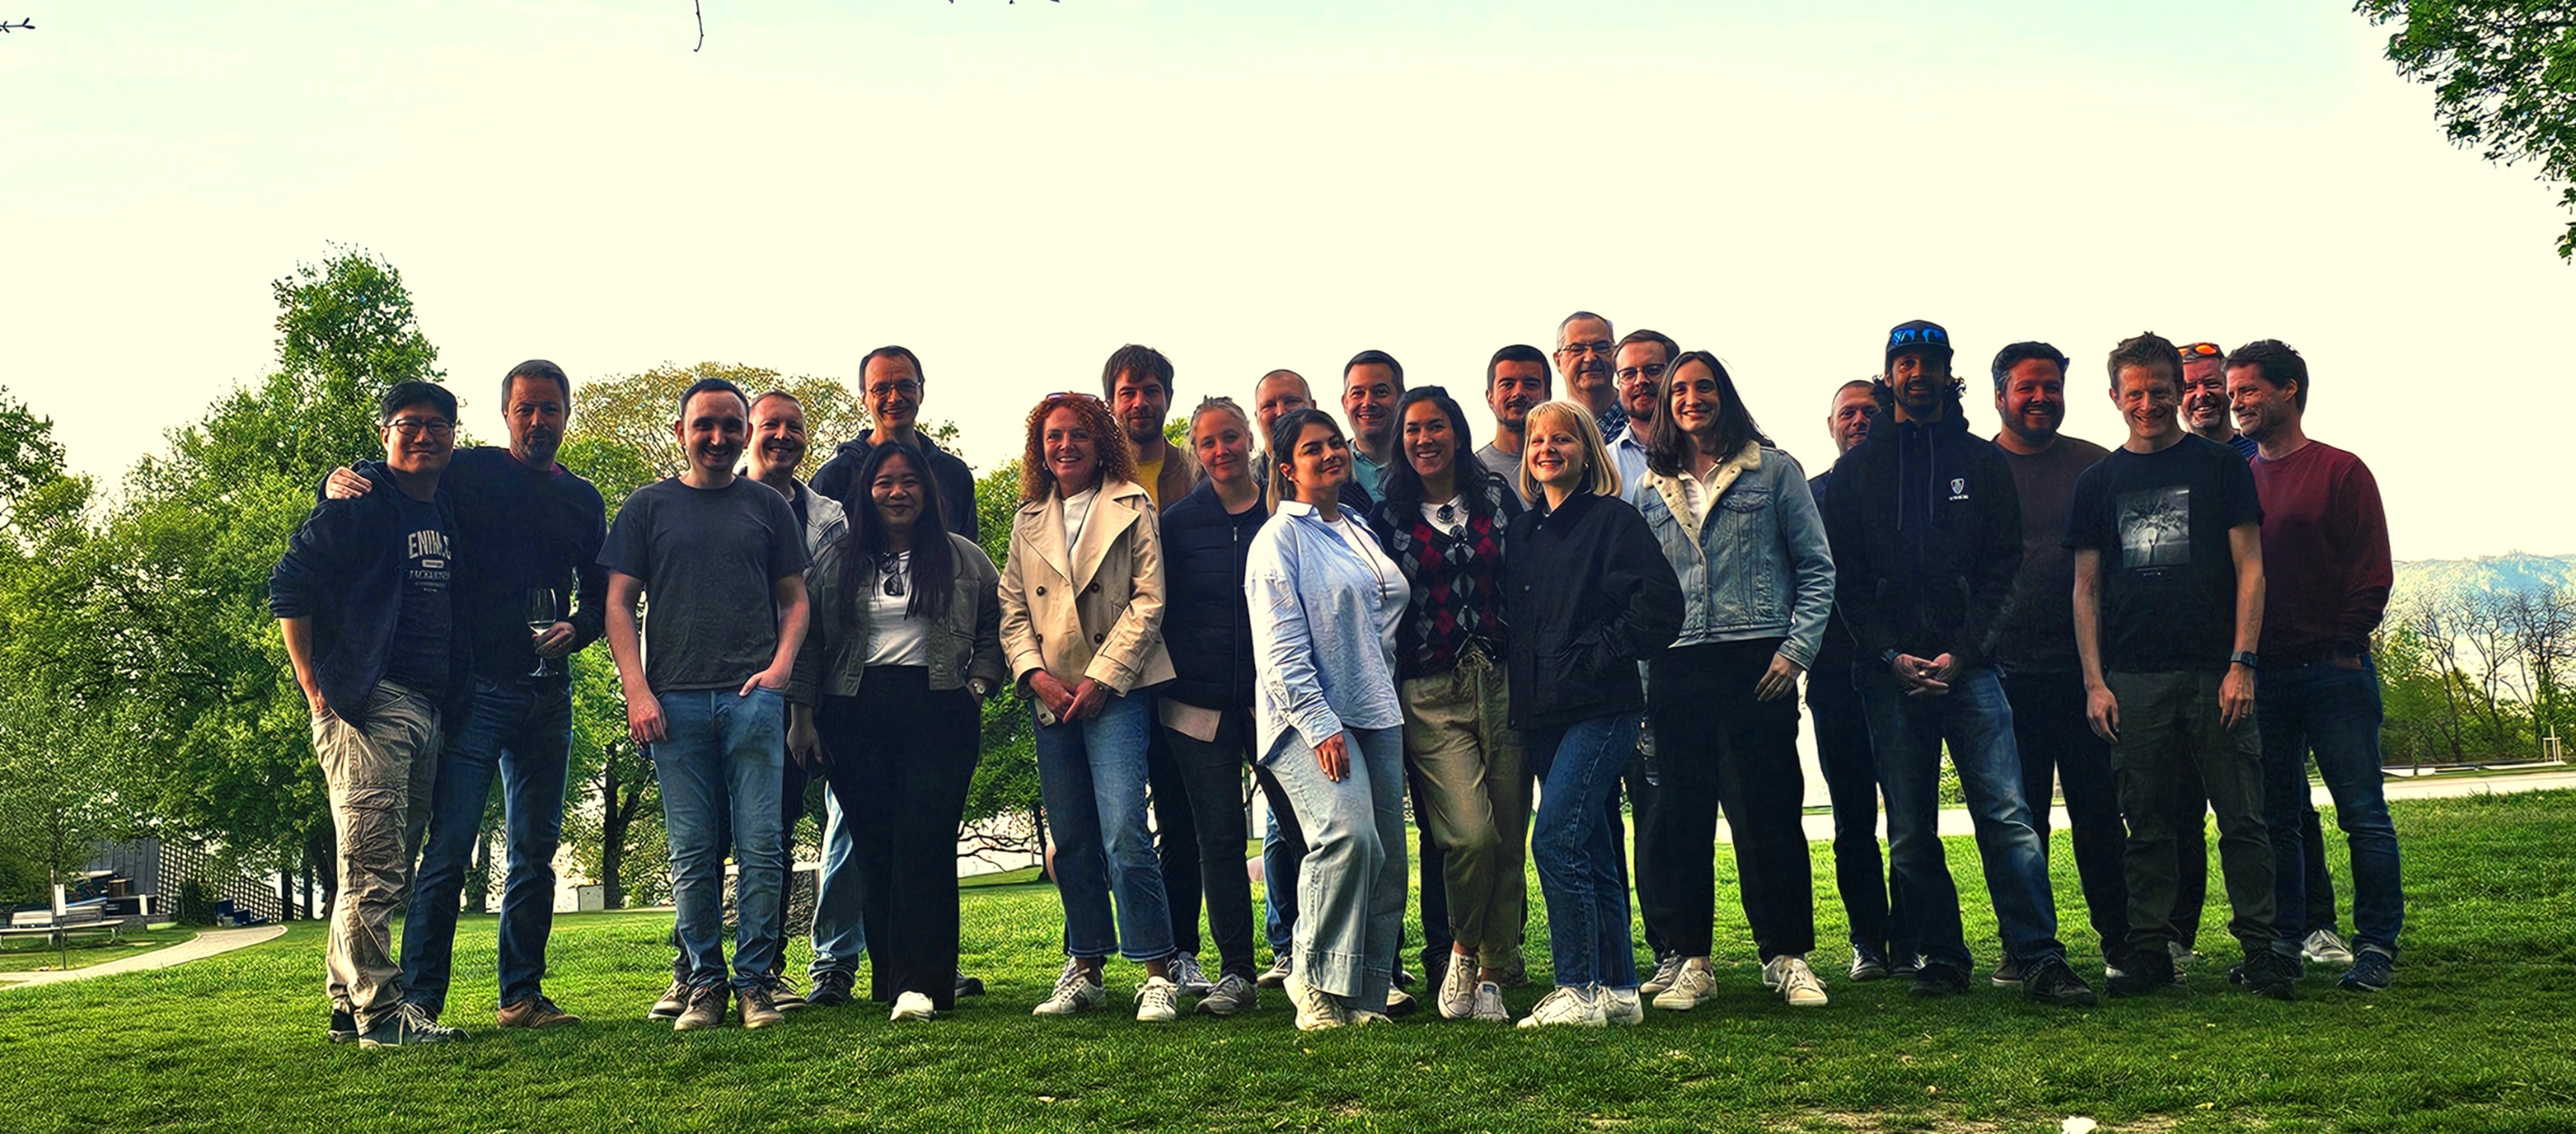
\includegraphics[width=0.8\textwidth]{./content/img/ProjectManagement/BizDevOps_Team.png}
    \caption{Picture of DWH LS OPS team}
    \label{fig:dwhlsops_apero}
\end{figure}

Within the Swiss Post this team is also referred as a \textbf{Busi}ness \textbf{Dev}elopment \textbf{Op}eration\textbf{s} (\gls{BizDevOps})  team, because it contains all required personnel, to create, deploy and maintain reporting solutions. This starts with \gls{businessanalyst}s to evaluate existing reports and their usage, and to document and specify them for further updates or re-engineering. This continues through the implementation, which is carried out first by data engineers and then by business intelligence (\gls{BI}) engineers. Finally, the business side is involved in testing these reports and also serves as the main source when it comes to questions of how or what to implement. Due to the size of this team and the different responsibilities, the DWH LS OPS team consists of three separate sub-teams. These teams are ordered along the process of postal services as introduced in the full mail piece lifecycle being: Receiving, Sorting, Transport, Customs clearance (German acronym is \gls{ASTV}), \textbf{D}elivery \textbf{\&} \textbf{F}inance (\gls{DandF}), and finally the planning focused Parcel Volume Planning and Forecasting (german acronym is \gls{MPP}).

\begin{figure}[H]
    \centering
    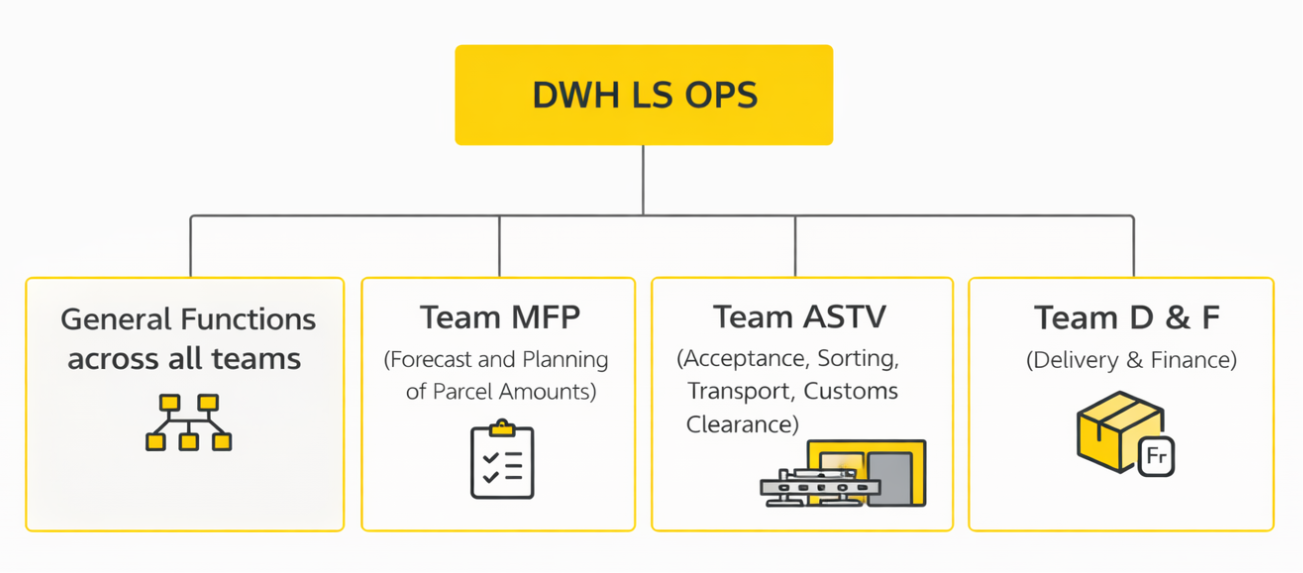
\includegraphics[width=0.8\textwidth]{./content/img/ProjectManagement/BizDevOps_OrgChart.png}
    \caption{Team and sub-team organisation}
    \label{fig:dwhlsops_member_names}
\end{figure}

\subsubsection*{AWS modernisation team}
\label{sec:AWSmodernisationteam}
Swiss Post is currently in a process the modernisation of the AWS cloud environment, which the Swiss Post itself describes as follows:

\textit{Swiss Post is currently pursuing a strategic modernisation of its AWS-based data lake with the objective of improving developer efficiency, increasing operational reliability, and establishing a modern, data-driven architecture. According to internal documentation, the initiative is aligned with defined key performance indicators and aims for completion by the end of the first quarter of 2026 \cite{SwissPostAWSModernization}.}

This modernisation is performed with the assistance of consultants as part of improving AWS usage in DWH LS OPS. The improvements are detailed in 15 \gls{KPI}s across topics such as \gls{AWSGlue} job optimisation and deployment pipeline improvements. With the assistance of the consultants, best practices are applied to the development of \gls{ETL}, as well as general improvements to deployment pipelines. Most importantly for this project, the initiative also includes \gls{DQM} improvements. As a reference, a screenshot of the Confluence landing page describing the initiative is shown below:

\begin{figure}[H]
    \centering
    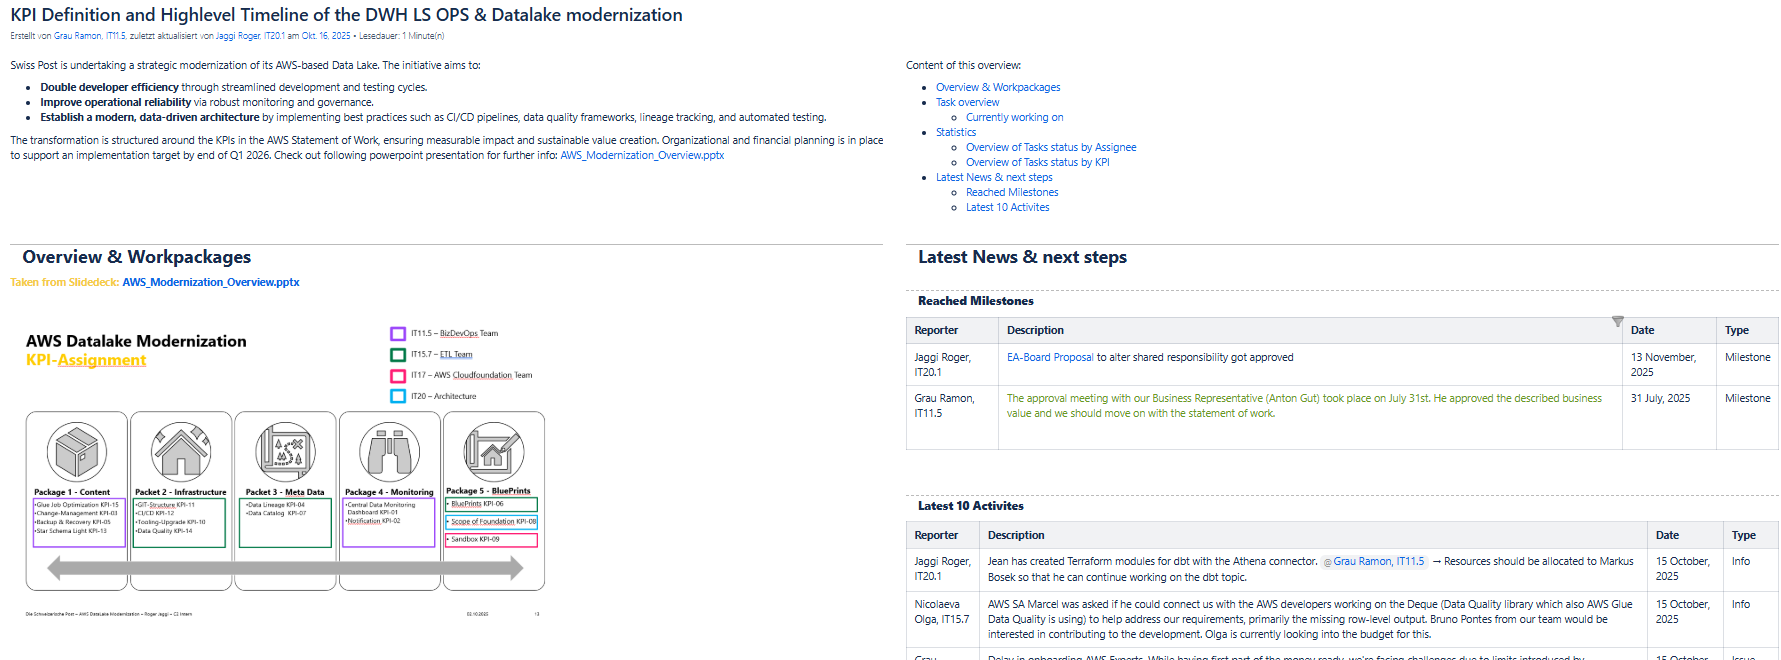
\includegraphics[width=0.8\textwidth]{./content/img/ProjectManagement/AWS_Modernisation_StartPage.png}
    \caption{The start page of the AWS modernisation, listing KPI and latest news}
    \label{fig:aws_modernisation_startpage}
\end{figure}

This team consists mainly of consultants with long-term experience in assisting companies in becoming proficient with AWS. They support data engineers at Swiss Post by improving existing code and reviewing it for potential enhancements. This is relevant for Swiss Post, as the development of the cloud infrastructure started without full architectural support and therefore has room for improvement.

\begin{figure}[H]
    \centering
    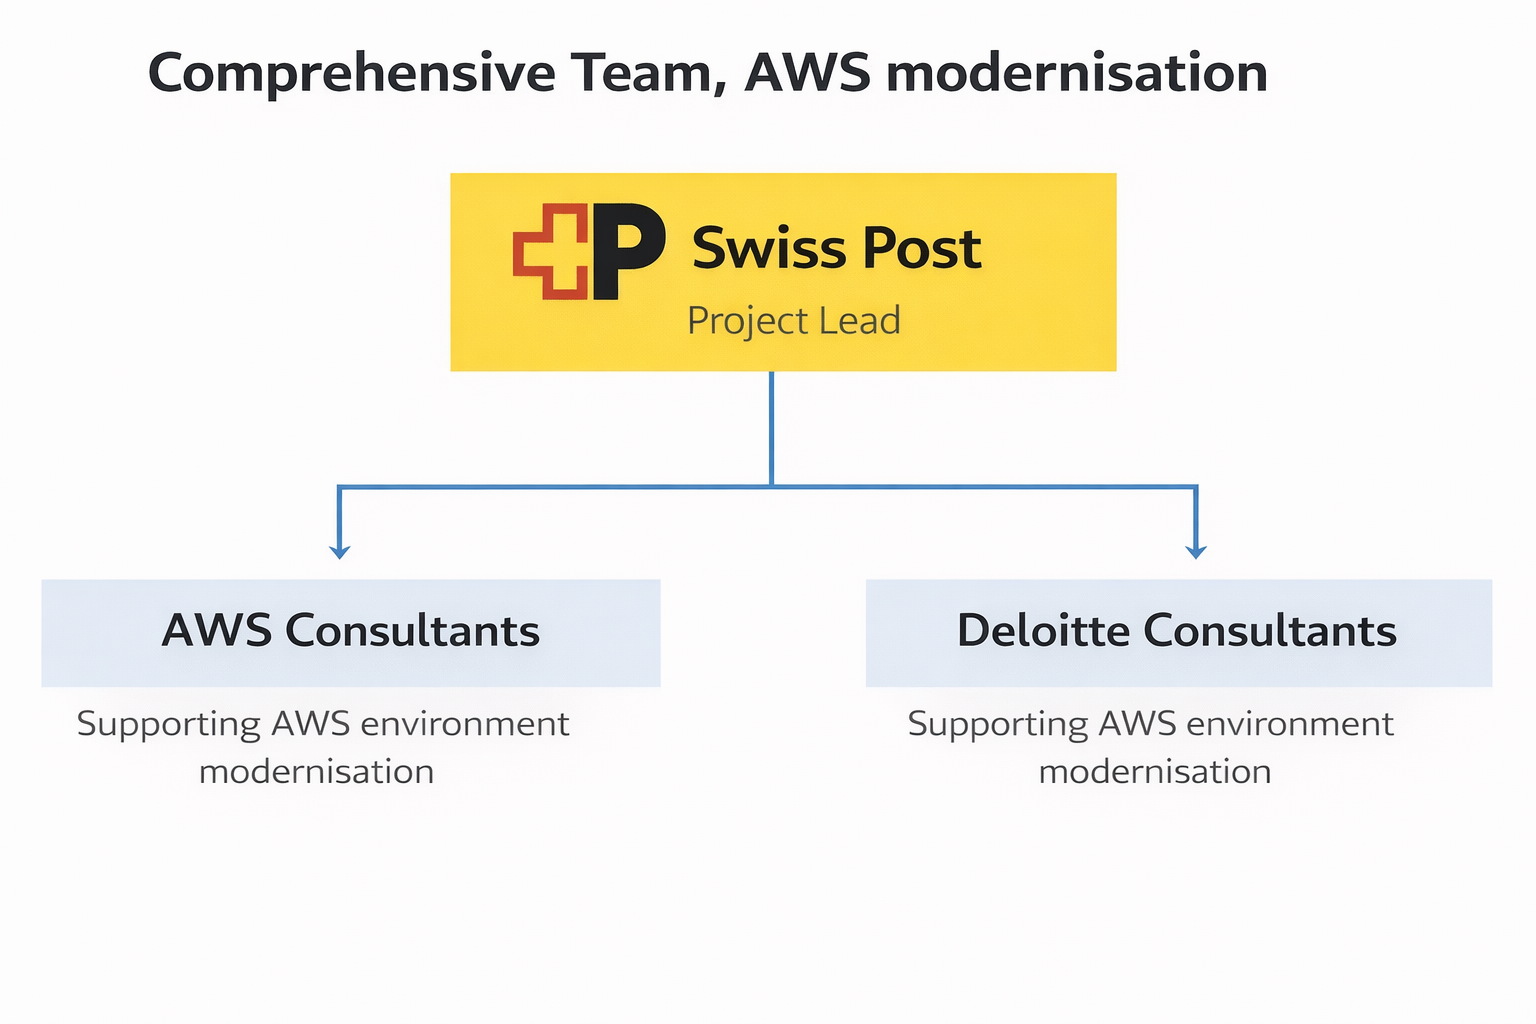
\includegraphics[width=0.8\textwidth]{./content/img/ProjectManagement/AWS_Modernisation_Setup.png}
    \caption{The team setup of the AWS modernisation}
    \label{fig:aws_modernisation_teammembers}
\end{figure}

\subsubsection*{DQM team}
\label{sec:DQMteam}
The third team relevant to the project is the \gls{DQM} team. The team serves KPI 14 Data Quality within the AWS modernisation. Their goal is described on Confluence as follows: specify, review, and implement an MVP to enable data scientists and ETL engineers to forward data quality measures to a monitoring dashboard for both business users and developers.

\begin{figure}[H]
    \centering
    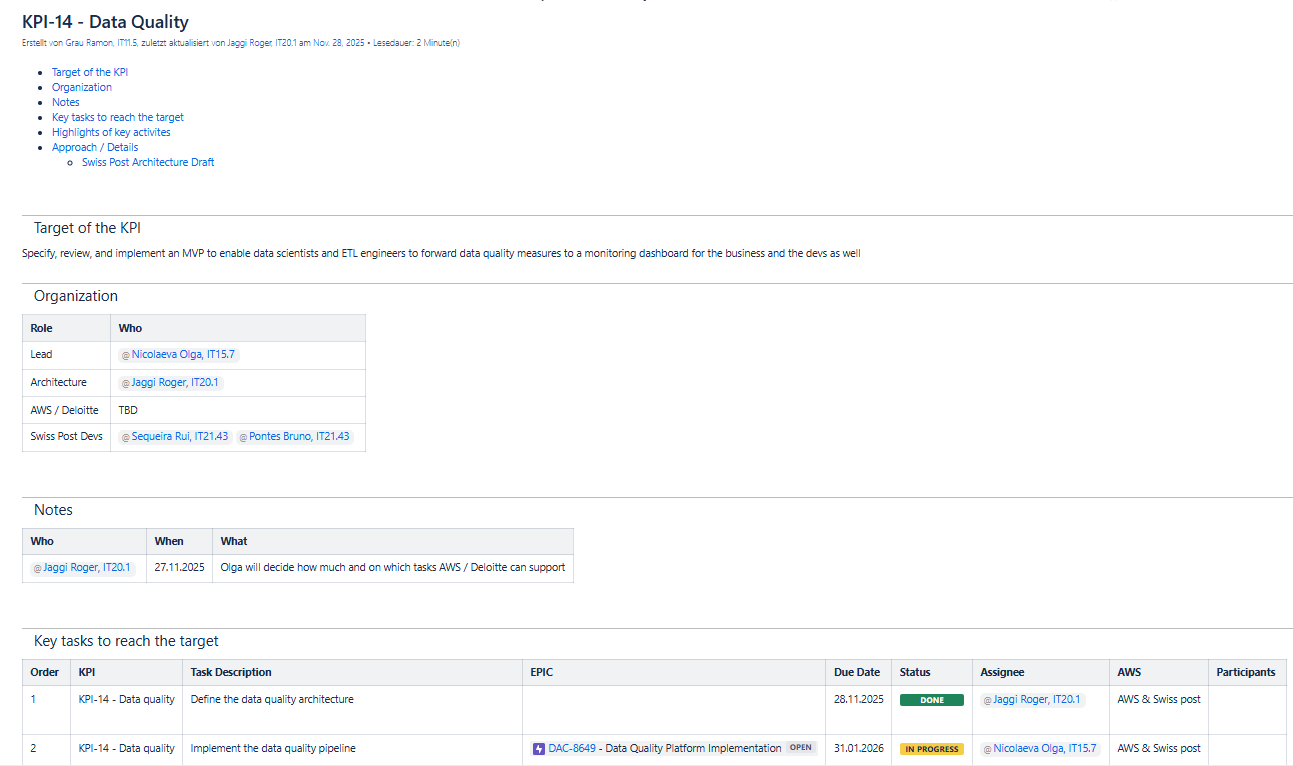
\includegraphics[width=0.8\textwidth]{./content/img/ProjectManagement/Startpage_DQM_KPI14.png}
    \caption{The KPI 14 Data Quality start page on DWH LS OPS Confluence}
    \label{fig:dwhlsops_kpi14_dqm}
\end{figure}

The team consists of three developers with the assistance of a lead data engineer. This setup ensures that the developers can deliver results efficiently, while the lead data engineer provides design guidance and solution structure.

\begin{figure}[H]
    \centering
    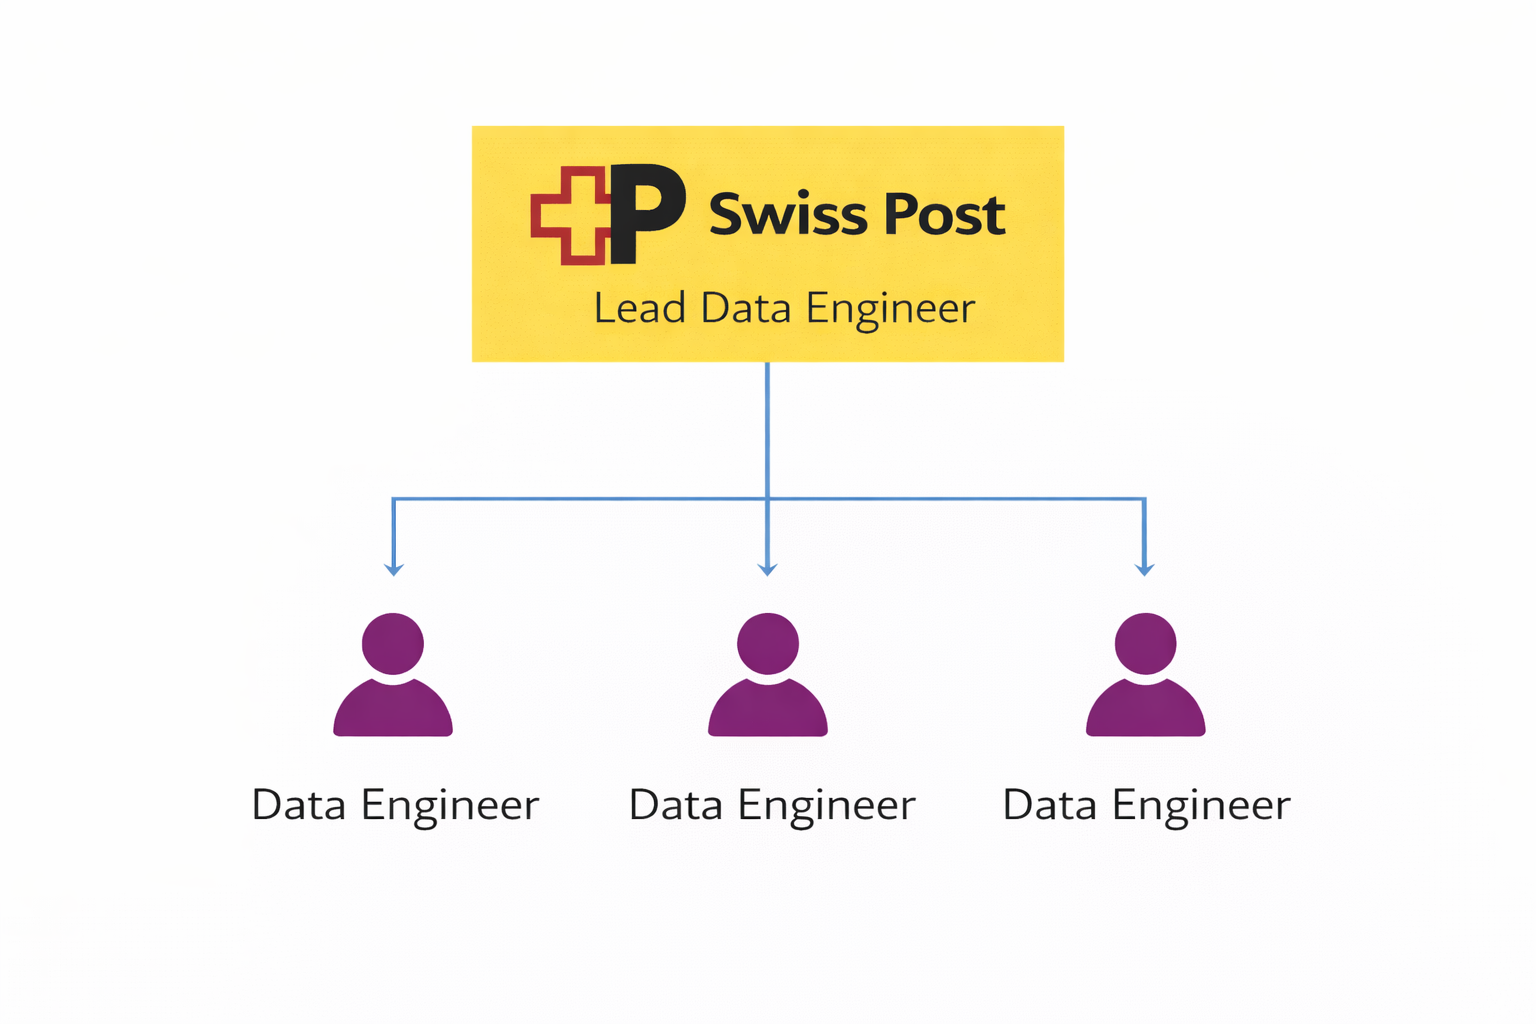
\includegraphics[width=0.8\textwidth]{./content/img/ProjectManagement/DQM_KPI14_Team_NoNames.png}
    \caption{The DQM team setup}
    \label{fig:dwhlsops_kpi14_team_dqm}
\end{figure}

\subsection*{Academic project team}
\label{sec:AcademicTeam}
The academic team consists of the author and the academic advisor. The author conducts the practical work, which includes analysis, implementation, and evaluation. The advisor provides expertise in the academic process and acts as a sparring partner regarding the writing process and project management, offering methodological and academic supervision.

\begin{figure}[H]
    \centering
    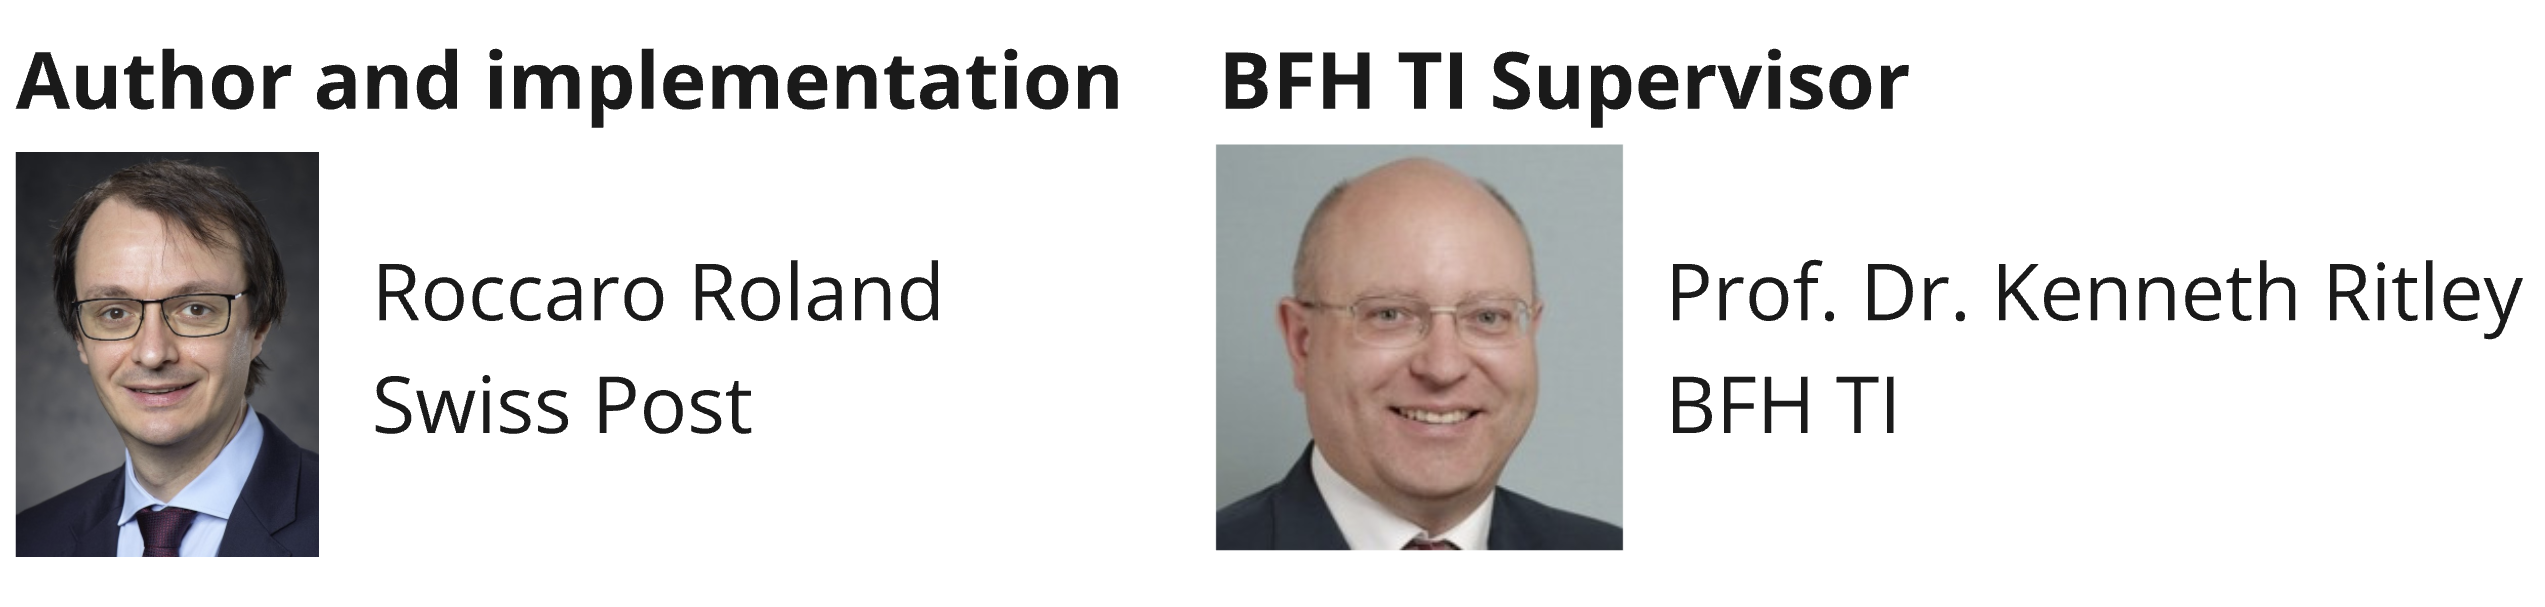
\includegraphics[width=0.8\textwidth]{./content/img/ProjectManagement/ProjectTeam_clean.png}
    \caption{The academic team setup}
    \label{fig:academic_team}
\end{figure}

\section{Project management methodologies}
\label{ProjMgmtMethods}
This section details how the different teams manage themselves. This is done for reasons of transparency, so that the reader understands which project management methods the individual teams use. This highlights an additional level of complexity in the working environment. Not all teams are addressed in every subsection, as the project team was not involved in all teams’ methods to the same depth. First, project management methods are highlighted, followed by the different timeline management approaches. In the following figure, the different boards and management methods are aligned around the central academic team to illustrate the broad set of methods.

\begin{figure}[H]
    \centering
    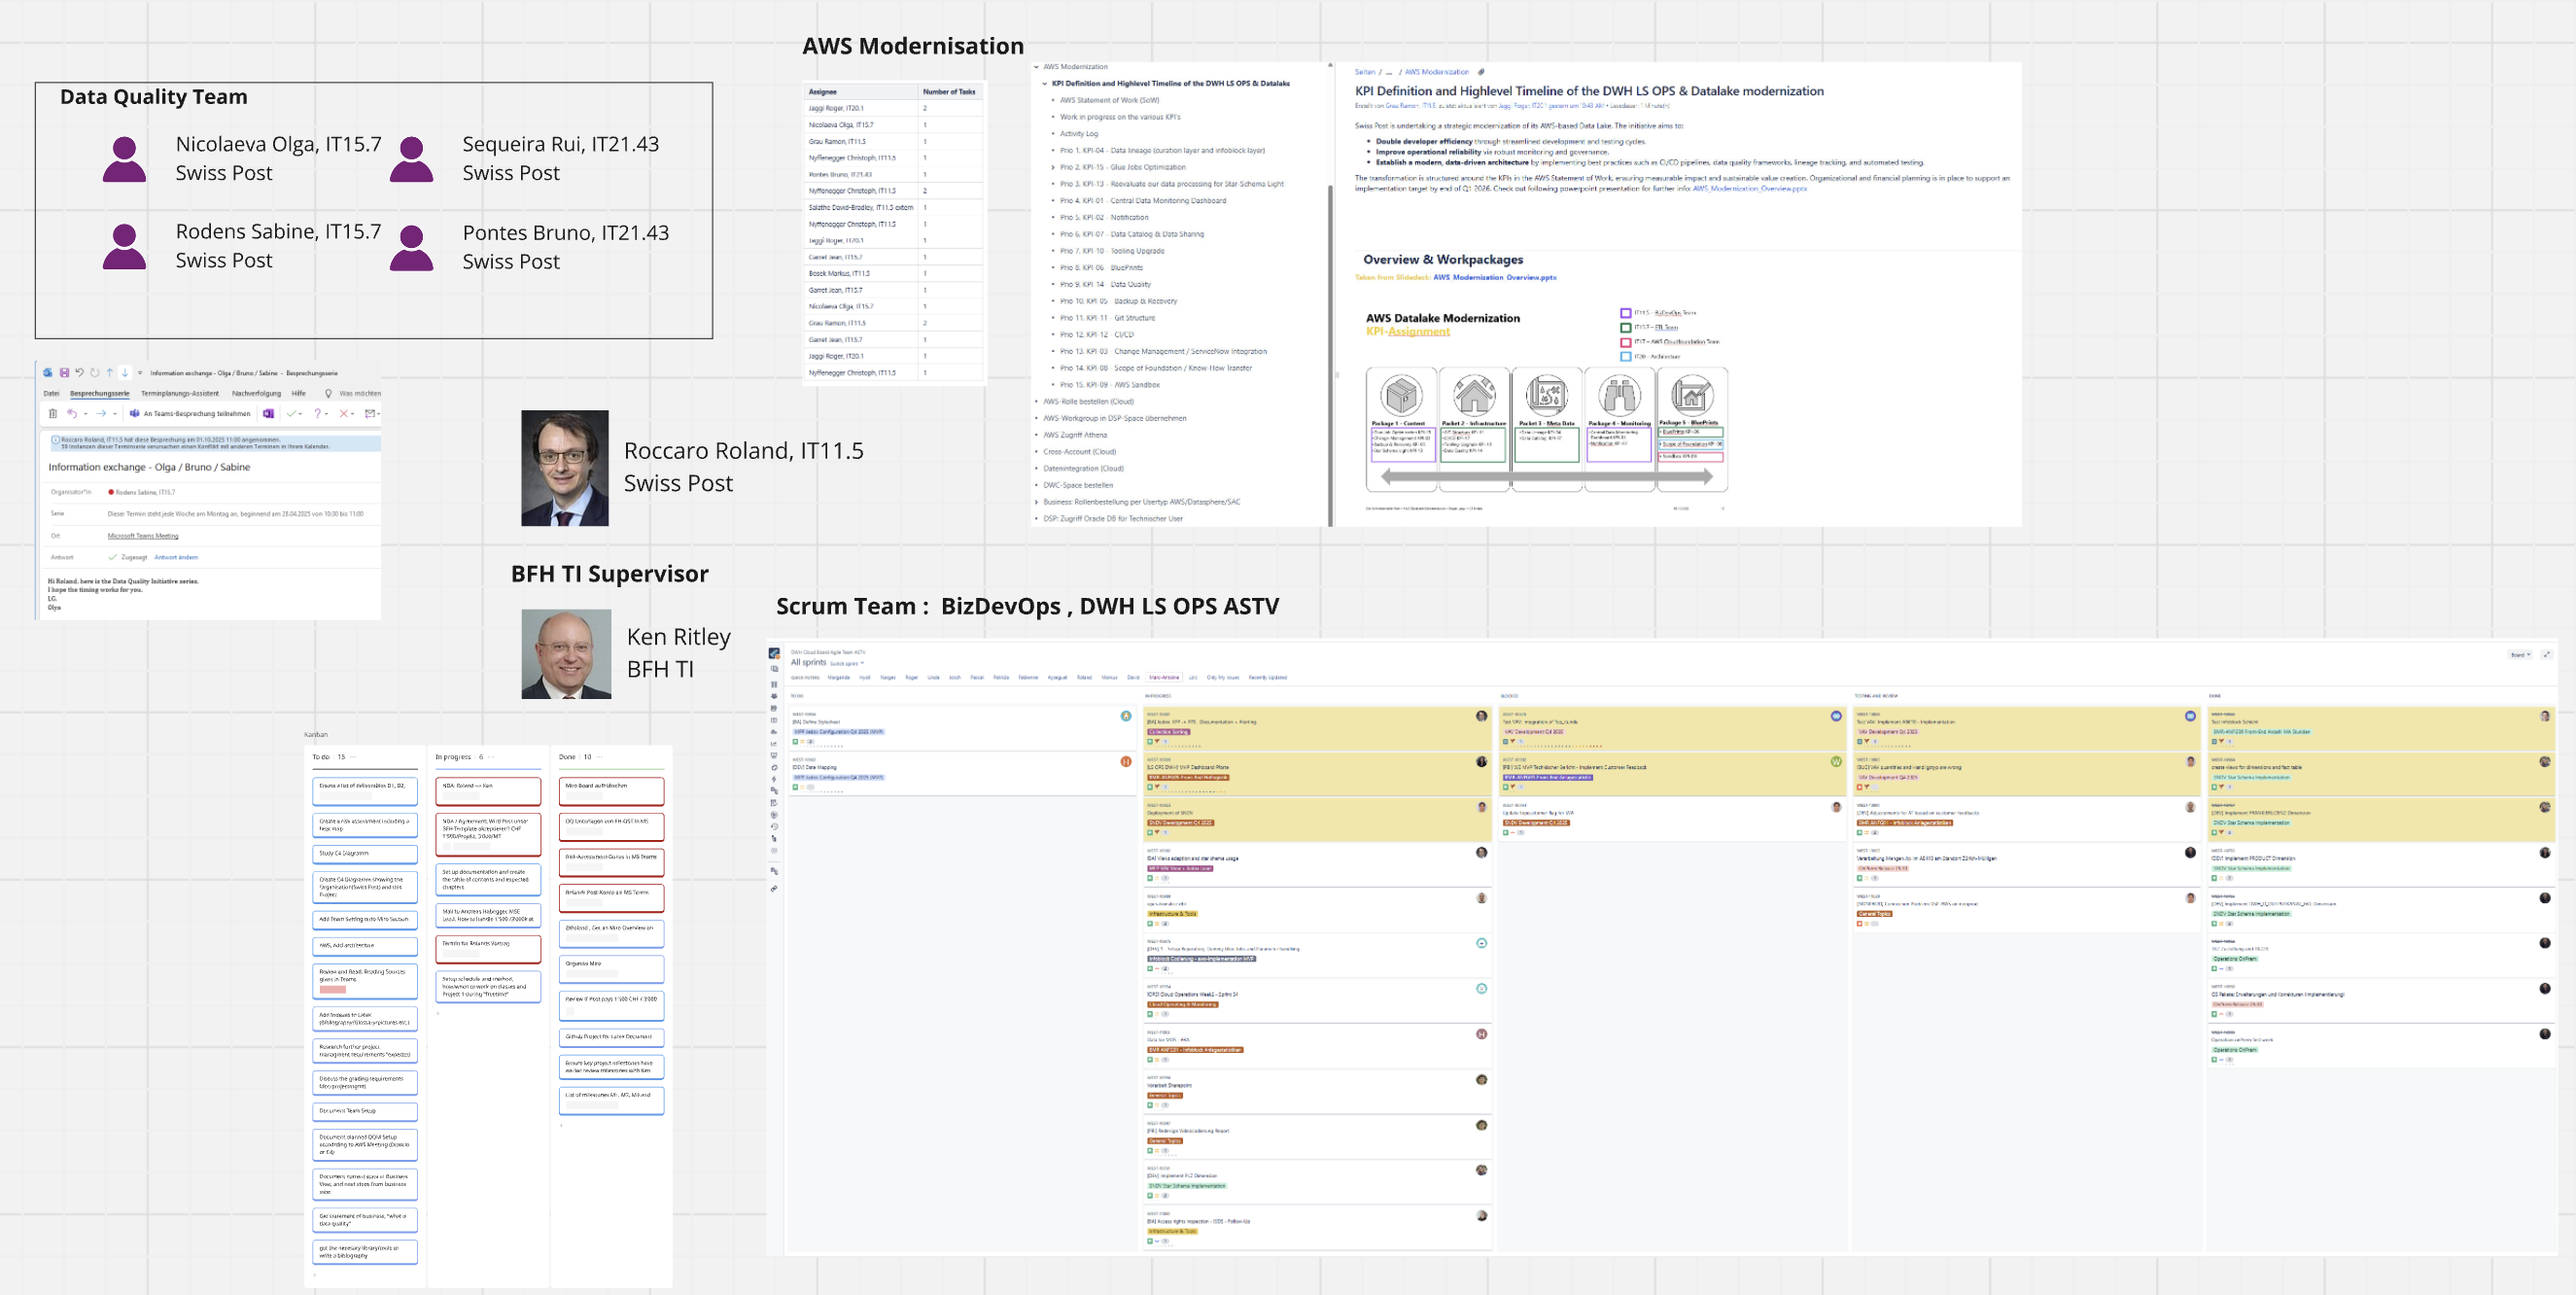
\includegraphics[width=0.8\textwidth]{./content/img/PostTeams_Tools.png}
    \caption{All methods on one picture showing their diversity}
    \label{fig:projmgmt_methods_one_pic}
\end{figure}

\subsection*{Project management}
Project management for this project consists of three main elements. These are Scrum, Kanban, and weekly meetings.

\subsubsection*{Scrum}
The \gls{DWHLSOPS} team is organised as a \gls{BizDevOps} \gls{scrum} team (see Section \ref{sec:DWHLSOPSTeam}). The AWS modernisation teams join these Scrum teams \ref{sec:AWSmodernisationteam}. The full set of rituals defined for Scrum is used, including daily meetings, sprint retrospectives, sprint planning held every two weeks, and reviews held every four weeks. In addition, a weekly Scrum meeting is held to maintain communication between the ASTV, D\&F, and MPP teams. The meetings are shown in the first screenshot, while the second illustrates a noteworthy team definition: the rules of engagement established for collaboration, which are a result of the retrospectives.


\begin{figure}[H]
    \centering
    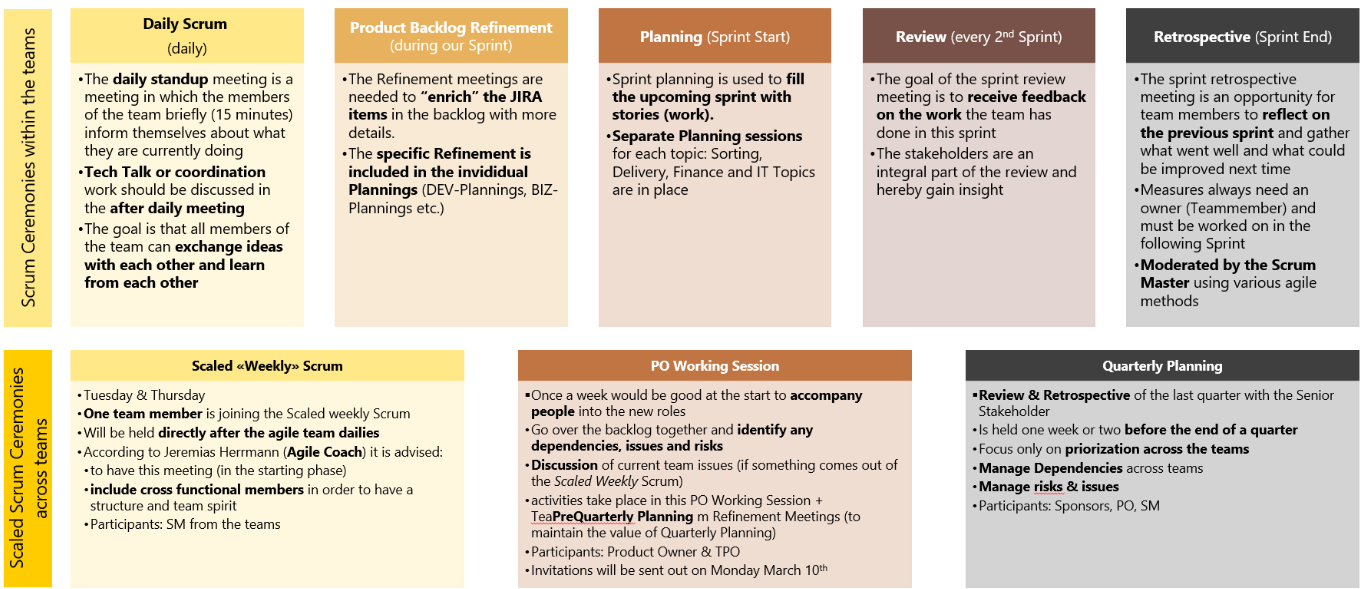
\includegraphics[width=0.8\textwidth]{./content/img/ProjectManagement/BizDevOps_ScrumCeremonies.PNG}
    \caption{Scrum ceremonies of DWH LS OPS  BizDevOps team}
    \label{fig:projmgmt_bizdevops_scrumMeetings}
\end{figure}

\begin{figure}[H]
    \centering
    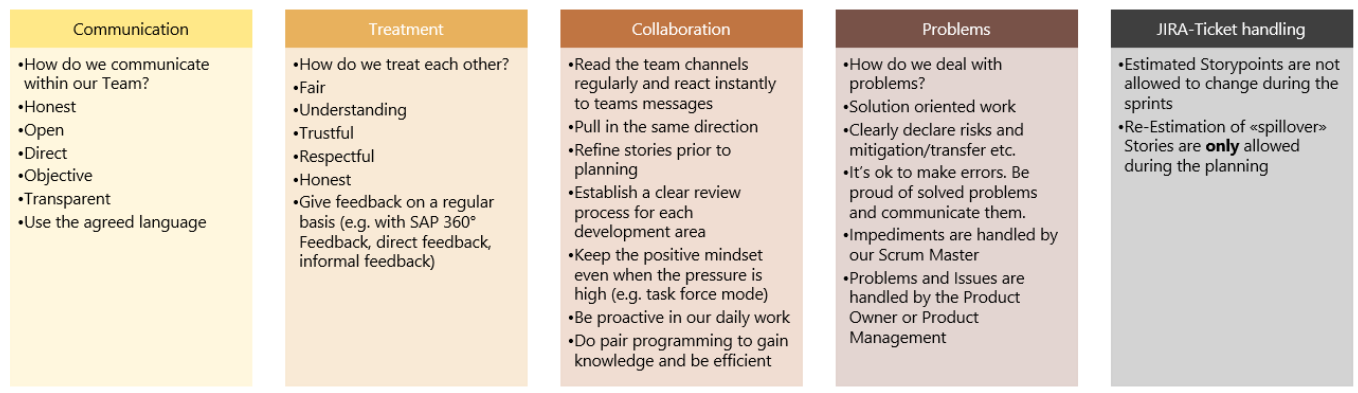
\includegraphics[width=0.8\textwidth]{./content/img/ProjectManagement/BizDevOps_RulesOfEngagement.png}
    \caption{Rules of engagement of DWH LS OPS  BizDevOps team}
    \label{fig:projmgmt_bizdevops_rulesofengagement}
\end{figure}

\subsubsection*{Weekly Meetings}
Contact with the \gls{DQM} team is handled using weekly meetings \ref{sec:DQMteam}. These serve as minimal update sessions during which weekly progress is communicated to all team members. While the developers in the DQM team are themselves also part of a Scrum team, their sprint management is out of scope.

\subsubsection*{Kanban}

The academic team handles tasks using a \gls{kanban} board \ref{sec:AcademicTeam}. The tasks are organised into three main columns. Both team members show their responsibilities on the Kanban board. The blue cards represent the author’s tasks, while the red cards represent the advisor’s tasks. The board is updated frequently and is reviewed during the weekly Jour Fixe.

\begin{figure}[H]
    \centering
    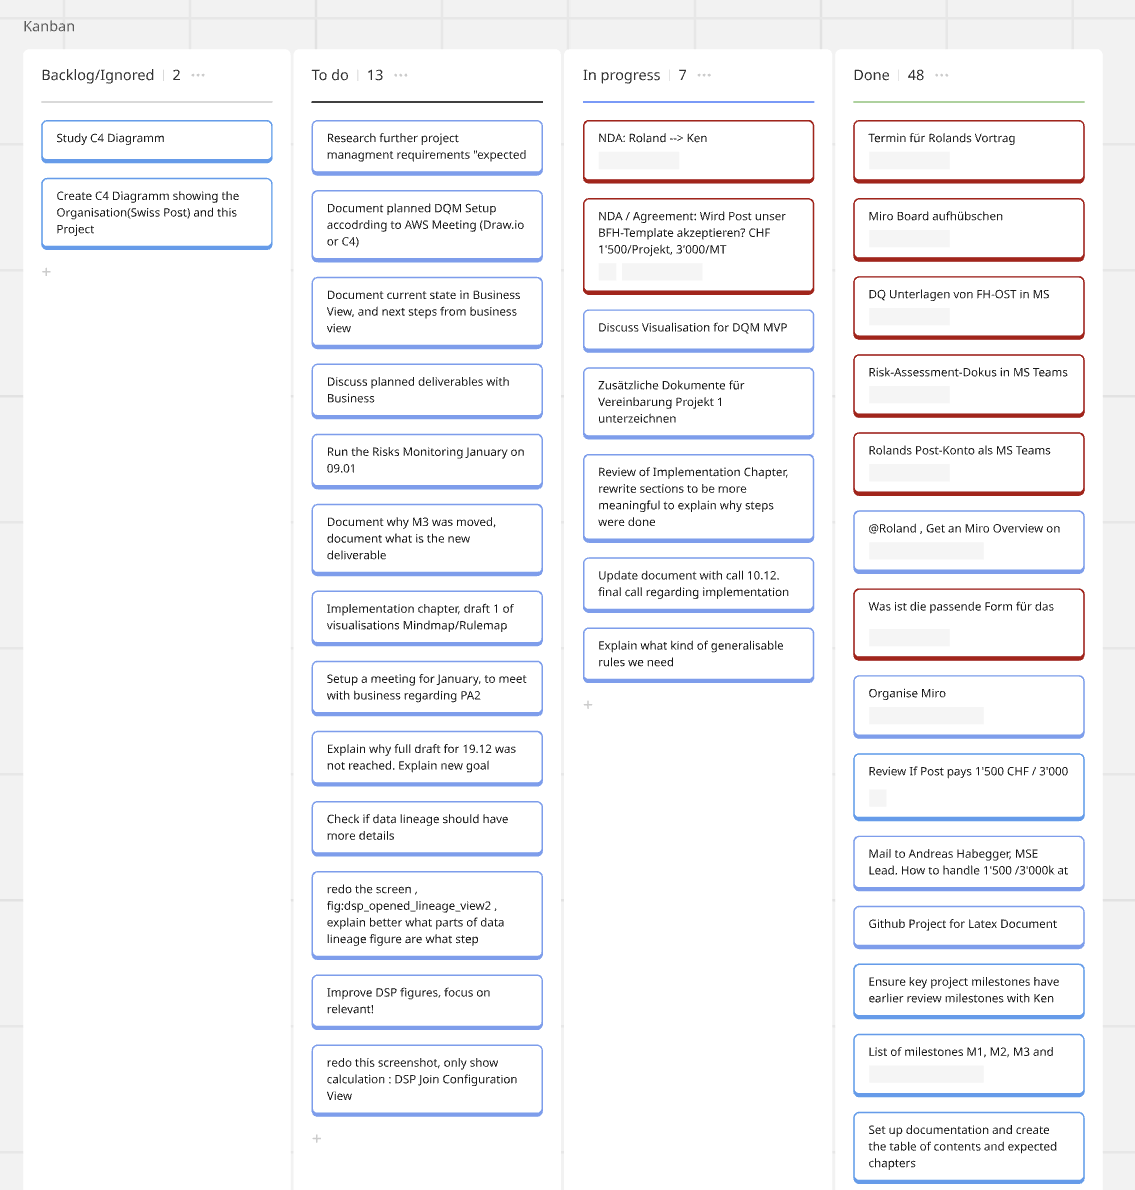
\includegraphics[width=0.8\textwidth]{./content/img/ProjectManagement/Academic_Kanban.png}
    \caption{Kanban board of Academic team}
    \label{fig:projmgmt_academic_kanban}
\end{figure}

\subsubsection*{Jour Fixe}

The academic team holds a \gls{JourFixe} every week \ref{sec:AcademicTeam}. This serves to maintain close communication and functions as a check-up meeting. Each meeting follows a defined structure; as an example, the meeting held on 15.12.2025 is described below.

\begin{itemize}
    \item Project check-in and clarification of objectives
    \item Overview of the project and completed deliverables
    \item Current deliverable in progress
    \item Status of milestones
    \item Changes needed to the updated Project 1 description
    \item Questions regarding Project 2
    \item Other topics
\end{itemize}

First, a general introduction to the project is provided to serve as a check-in and to allow participants to focus on the project. Second, the deliverables currently being worked on are listed based on the deliverables overview. Third, the status of the milestones is reviewed. Fourth, this is followed by individual agenda items, which can differ from meeting to meeting. In this meeting, these included updates to the Project 1 description required for agreement, as well as a check-in regarding topics and submission of Project 2. Finally, the meeting is closed with an open section in which any other relevant topics may be discussed. These meetings are documented in Miro (see below) and structured using a three-block template and are most often recorded using handwritten notes that are later uploaded.


 \begin{figure}[H]
    \centering
    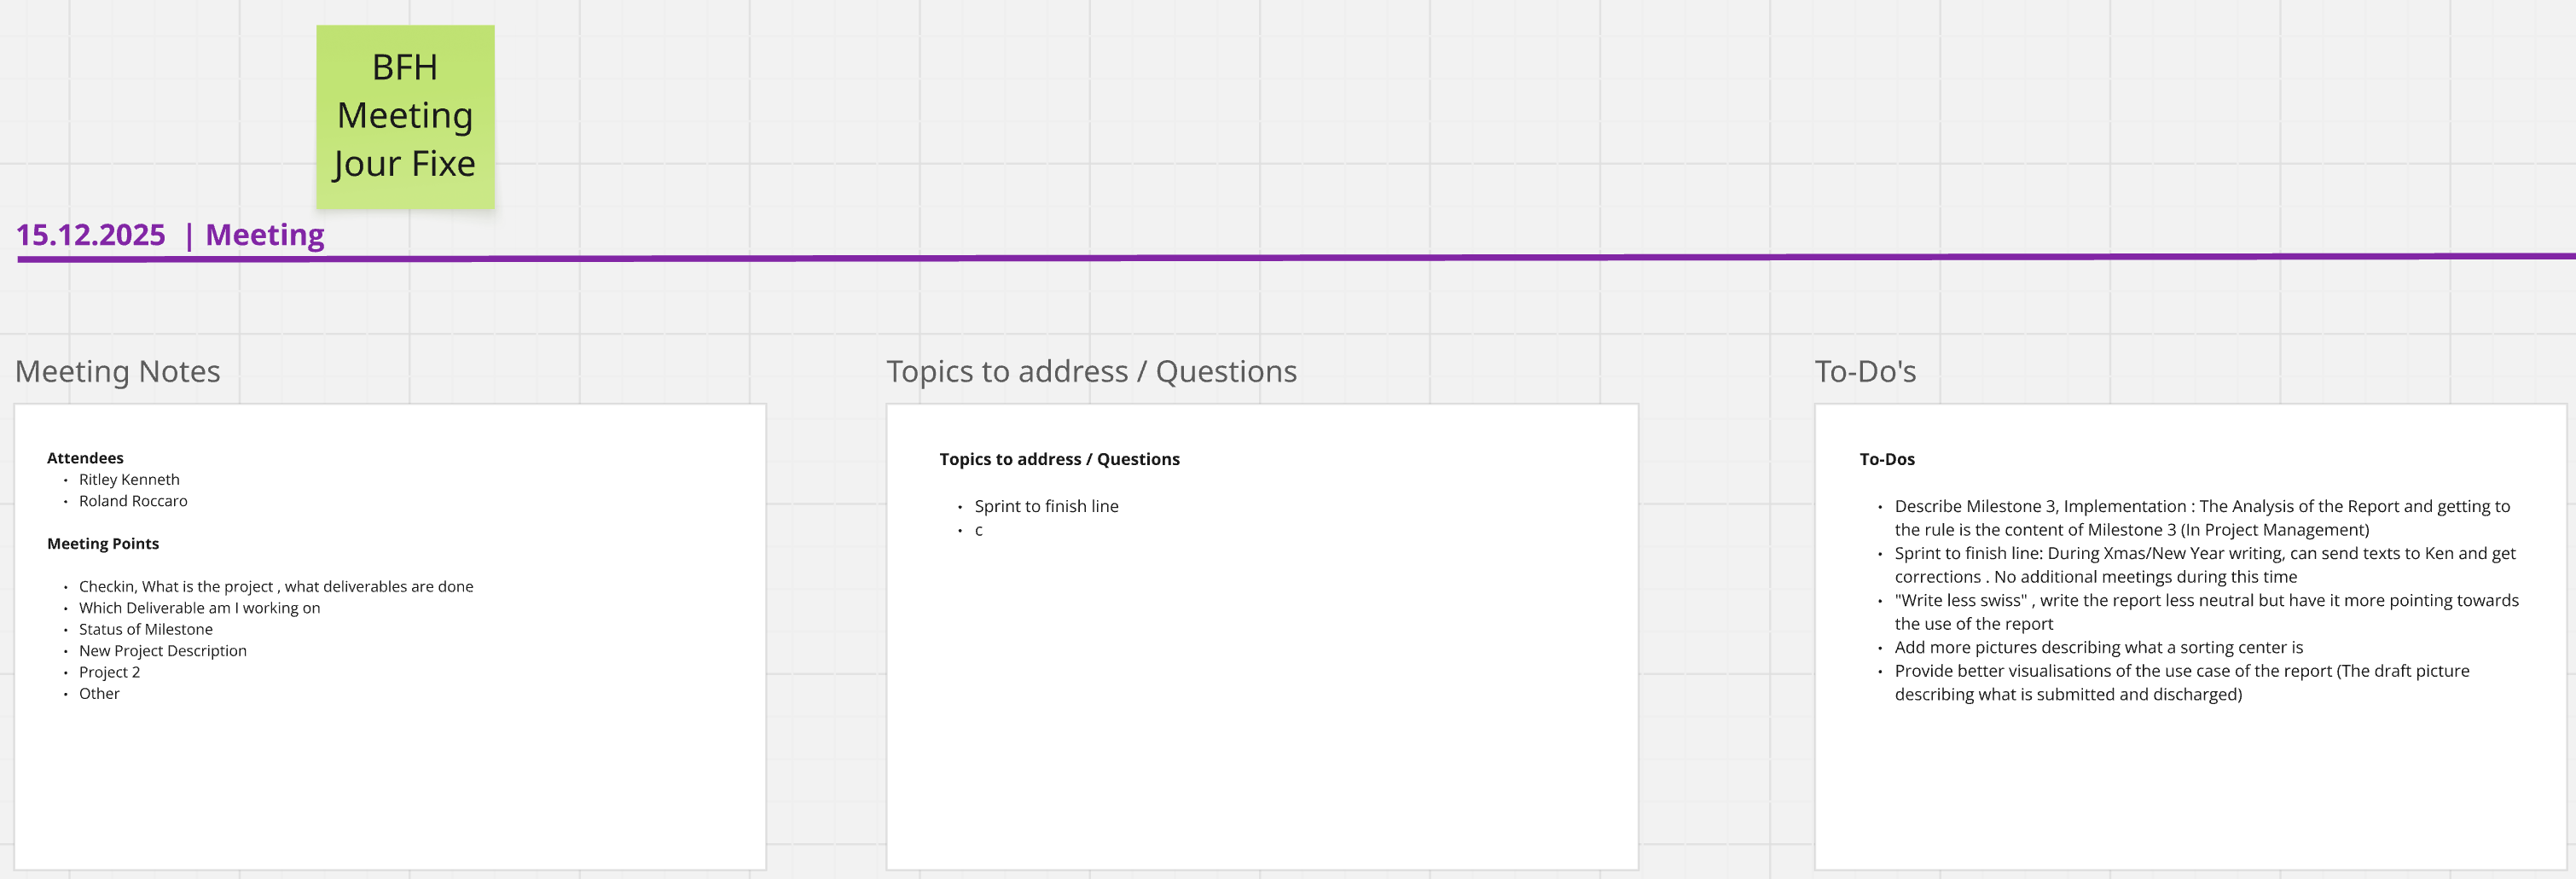
\includegraphics[width=0.8\textwidth]{./content/img/ProjectManagement/Academic_JourFixe.png}
    \caption{Jour Fixe of Academic team, meeting structure and rework}
    \label{fig:jour_fixe_academic_structure}
\end{figure}

\begin{figure}[H]
    \centering
    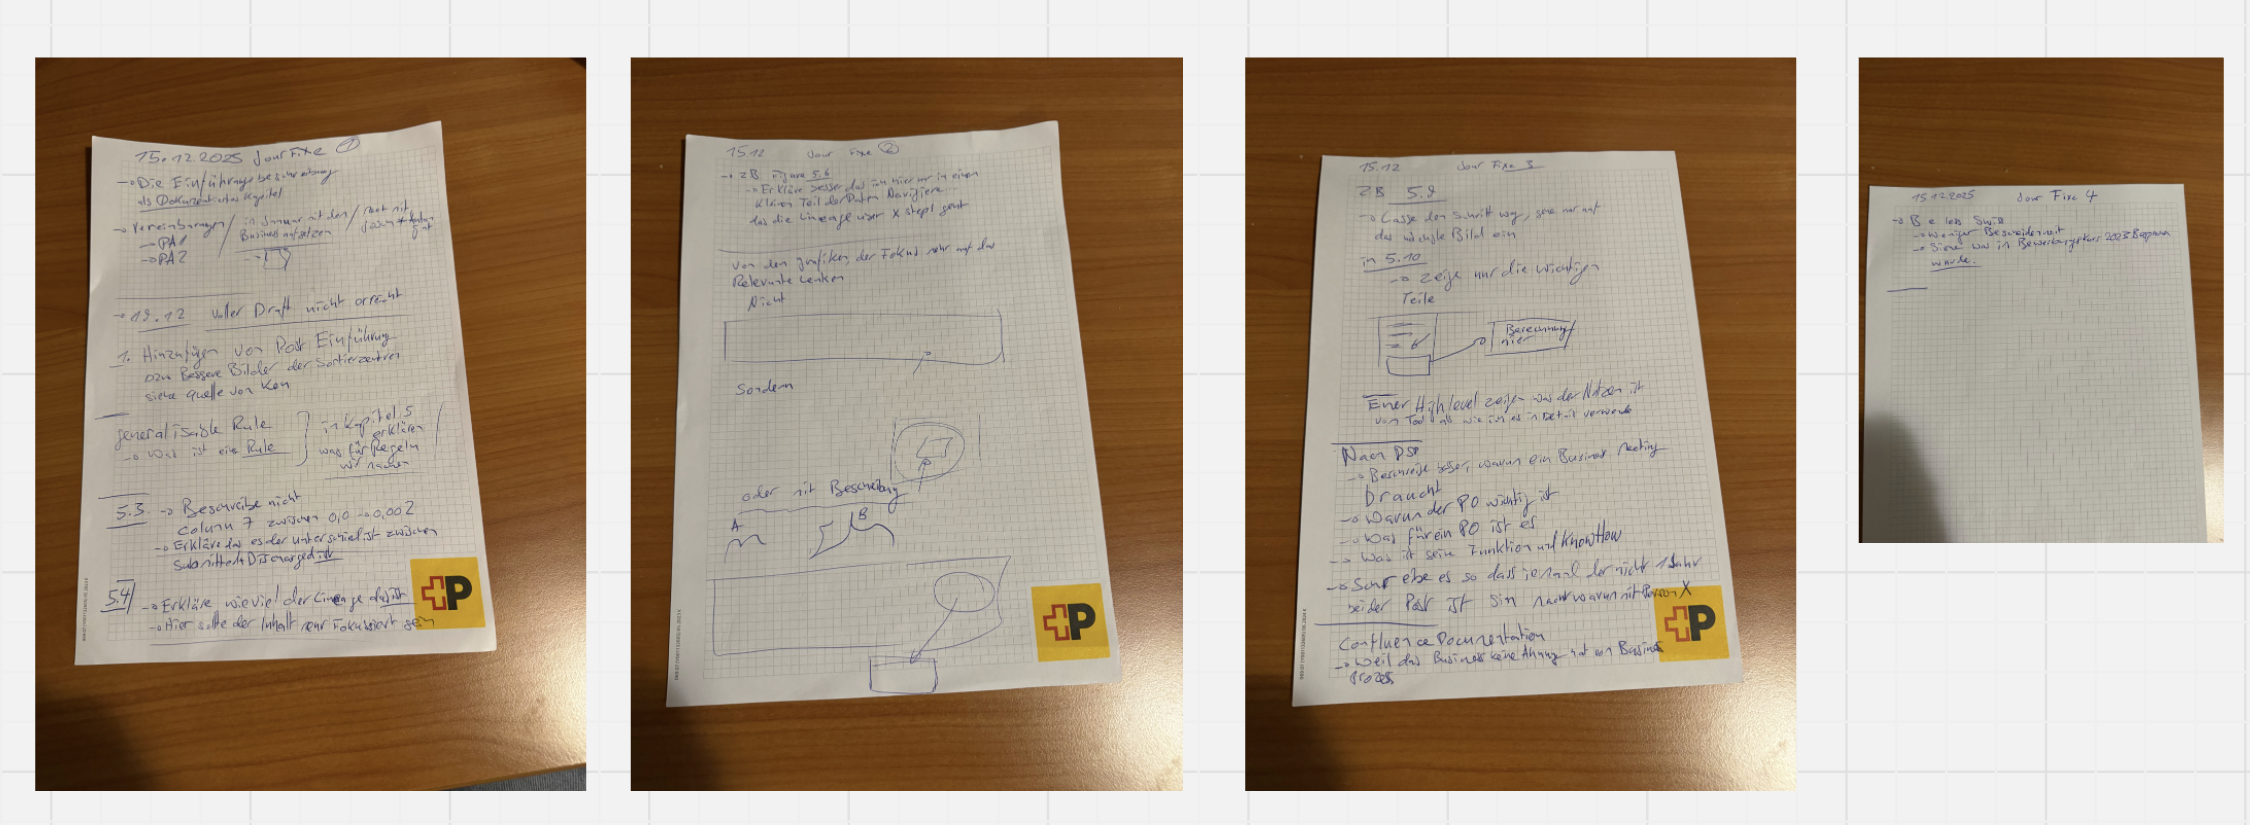
\includegraphics[width=0.8\textwidth]{./content/img/ProjectManagement/Academic_Jour_Fixe_Notes.png}
    \caption{Jour Fixe documentation of Academic team}
    \label{fig:jour_fixe_notes_academic}
\end{figure}

\subsection*{Timeline management}
Timeline management is performed in different ways by the teams. In this subsection, the planning of actions is described, as well as how staff availability is tracked.

\subsubsection*{Scrum Events}
The DWH LS OPS and the AWS modernisation teams use Scrum events to manage their timelines. Progress on stories is monitored in daily meetings, during which each team member updates the team on progress and issues and indicates whether assistance is needed or deviations from the previously planned approach are required. Sprints encompass the stories the team works on during a two-week cycle. During sprint planning, the stories for the next sprint are defined. The stories added to a sprint represent the commitment the team makes for the sprint, together with the sprint goal. Planning over longer time horizons is conducted through quarterly planning sessions. Every three months, all teams in DWH LS OPS plan which \gls{epic}s and how many story points should be completed. These quarterly planning sessions also serve to prioritise epics and allow higher management to introduce priorities.

\subsubsection*{Holidays}
Holidays are noted in the calendars used; this applies to the DWH LS OPS team as well as the academic team. In both cases, every holiday must be recorded with an absence notification. This allows other team members to quickly see whether a team member is available in the future and to adjust their planning accordingly, or to confirm in daily operations that the person is not available.

\subsubsection*{Milestones}
The academic team manages the planning of the overall project timeline using milestones. These milestones define timeframes during which a section or chapter may be worked on. For this project, the following milestones have been defined:

\begin{itemize}
    \item Milestone 1: Basics completed
    \item Milestone 2: Completion of main research
    \item Milestone 3: Code implementation completed
    \item Milestone 4: Bug fixing completed
    \item Milestone 5: Submission of the project document
    \item Milestone 6: Presentation prepared
\end{itemize}

First, the basics ready refers to tools to work with beeing available. This step includes setting up LateX, setting milestones, setup of basic tool structure and definition of way of work. Second the main research done refers to the end of the purely theoretical part and start towards the solution design and the subsequent implementation of it. This comprises the main literature research beeing done. Third, the code done refers to the implementation of the solution beeing done. After this point no new features are to be implemented. Fourth, bug fix done comprises all corrections that had to be performed so that the provided implementation works and technical debt amassed during development has been cleared. Fifth, the handin of the document is the final day according to the semester calender. Up to this date corrections to the document and finalisation can be provided. Sixth and final, the presentation must be ready latest by this date. After this some finetuning can be performed but the main content needs to be set.

The milestones were set to structure the work blocks, but primarily to define how much effort should be invested in each individual block. The time allocated per block is not estimated in terms of how long a task is expected to take. Instead, it is defined by how much time the team is willing to invest in a topic in order to ensure sufficient capacity for subsequent tasks. For example, documenting the Swiss Post environment could have taken two to three weeks; however, only three days were intentionally allocated to this task.

\subsubsection*{Deviations and Unavailabilities}
The academic team tracked deviations from milestones or Jour Fixe meetings. This served transparency and traceability. For this use case, the dates of all Jour Fixe meetings were planned in advance. If a meeting had to be rescheduled, this was noted in the calendar. In the case of shifted milestones, these changes also had to be documented in the calendar, including the reasoning for why a milestone was not achieved or had to be moved. In the Results chapter, deviations from the planned milestones are documented.
\section{Tools to support the project management}
\label{ProjMgmtTools}
This section lists the tools used during the project for reasons of transparency. It also allows the reader to evaluate different ways in which these tools can be used. 

\subsection*{Miro}
\label{ProjMgmtToolMiro}
Miro is part of the toolset of both the academic team and the Swiss Post teams. However, in this project, it was used only by the academic team. The reason for using Miro is that it is a lightweight tool that allows combining different data structures on a single board. Miro provides an infinite canvas on which a wide variety of information can be placed. The information can be structured and easily rearranged to regroup related elements. This allows the tool to be used both for early documentation of information and for later restructuring when additional ideas emerge, particularly in the context of long-term documentation. The ability to restructure information visually supports the decomposition and understanding of complex environments.

A full set of screenshots illustrating changes on the Miro board has been moved to the Annex, while the final one is included here (Appendix \ref{apendixMiroUsage}). The following screenshot represents the Miro board during the finalisation of the document, zoomed out so that all elements are visible. While this view prevents individual details from being seen, some relevant parts are shown in detail in the following subsubsections.

\begin{figure}[H]
    \centering
    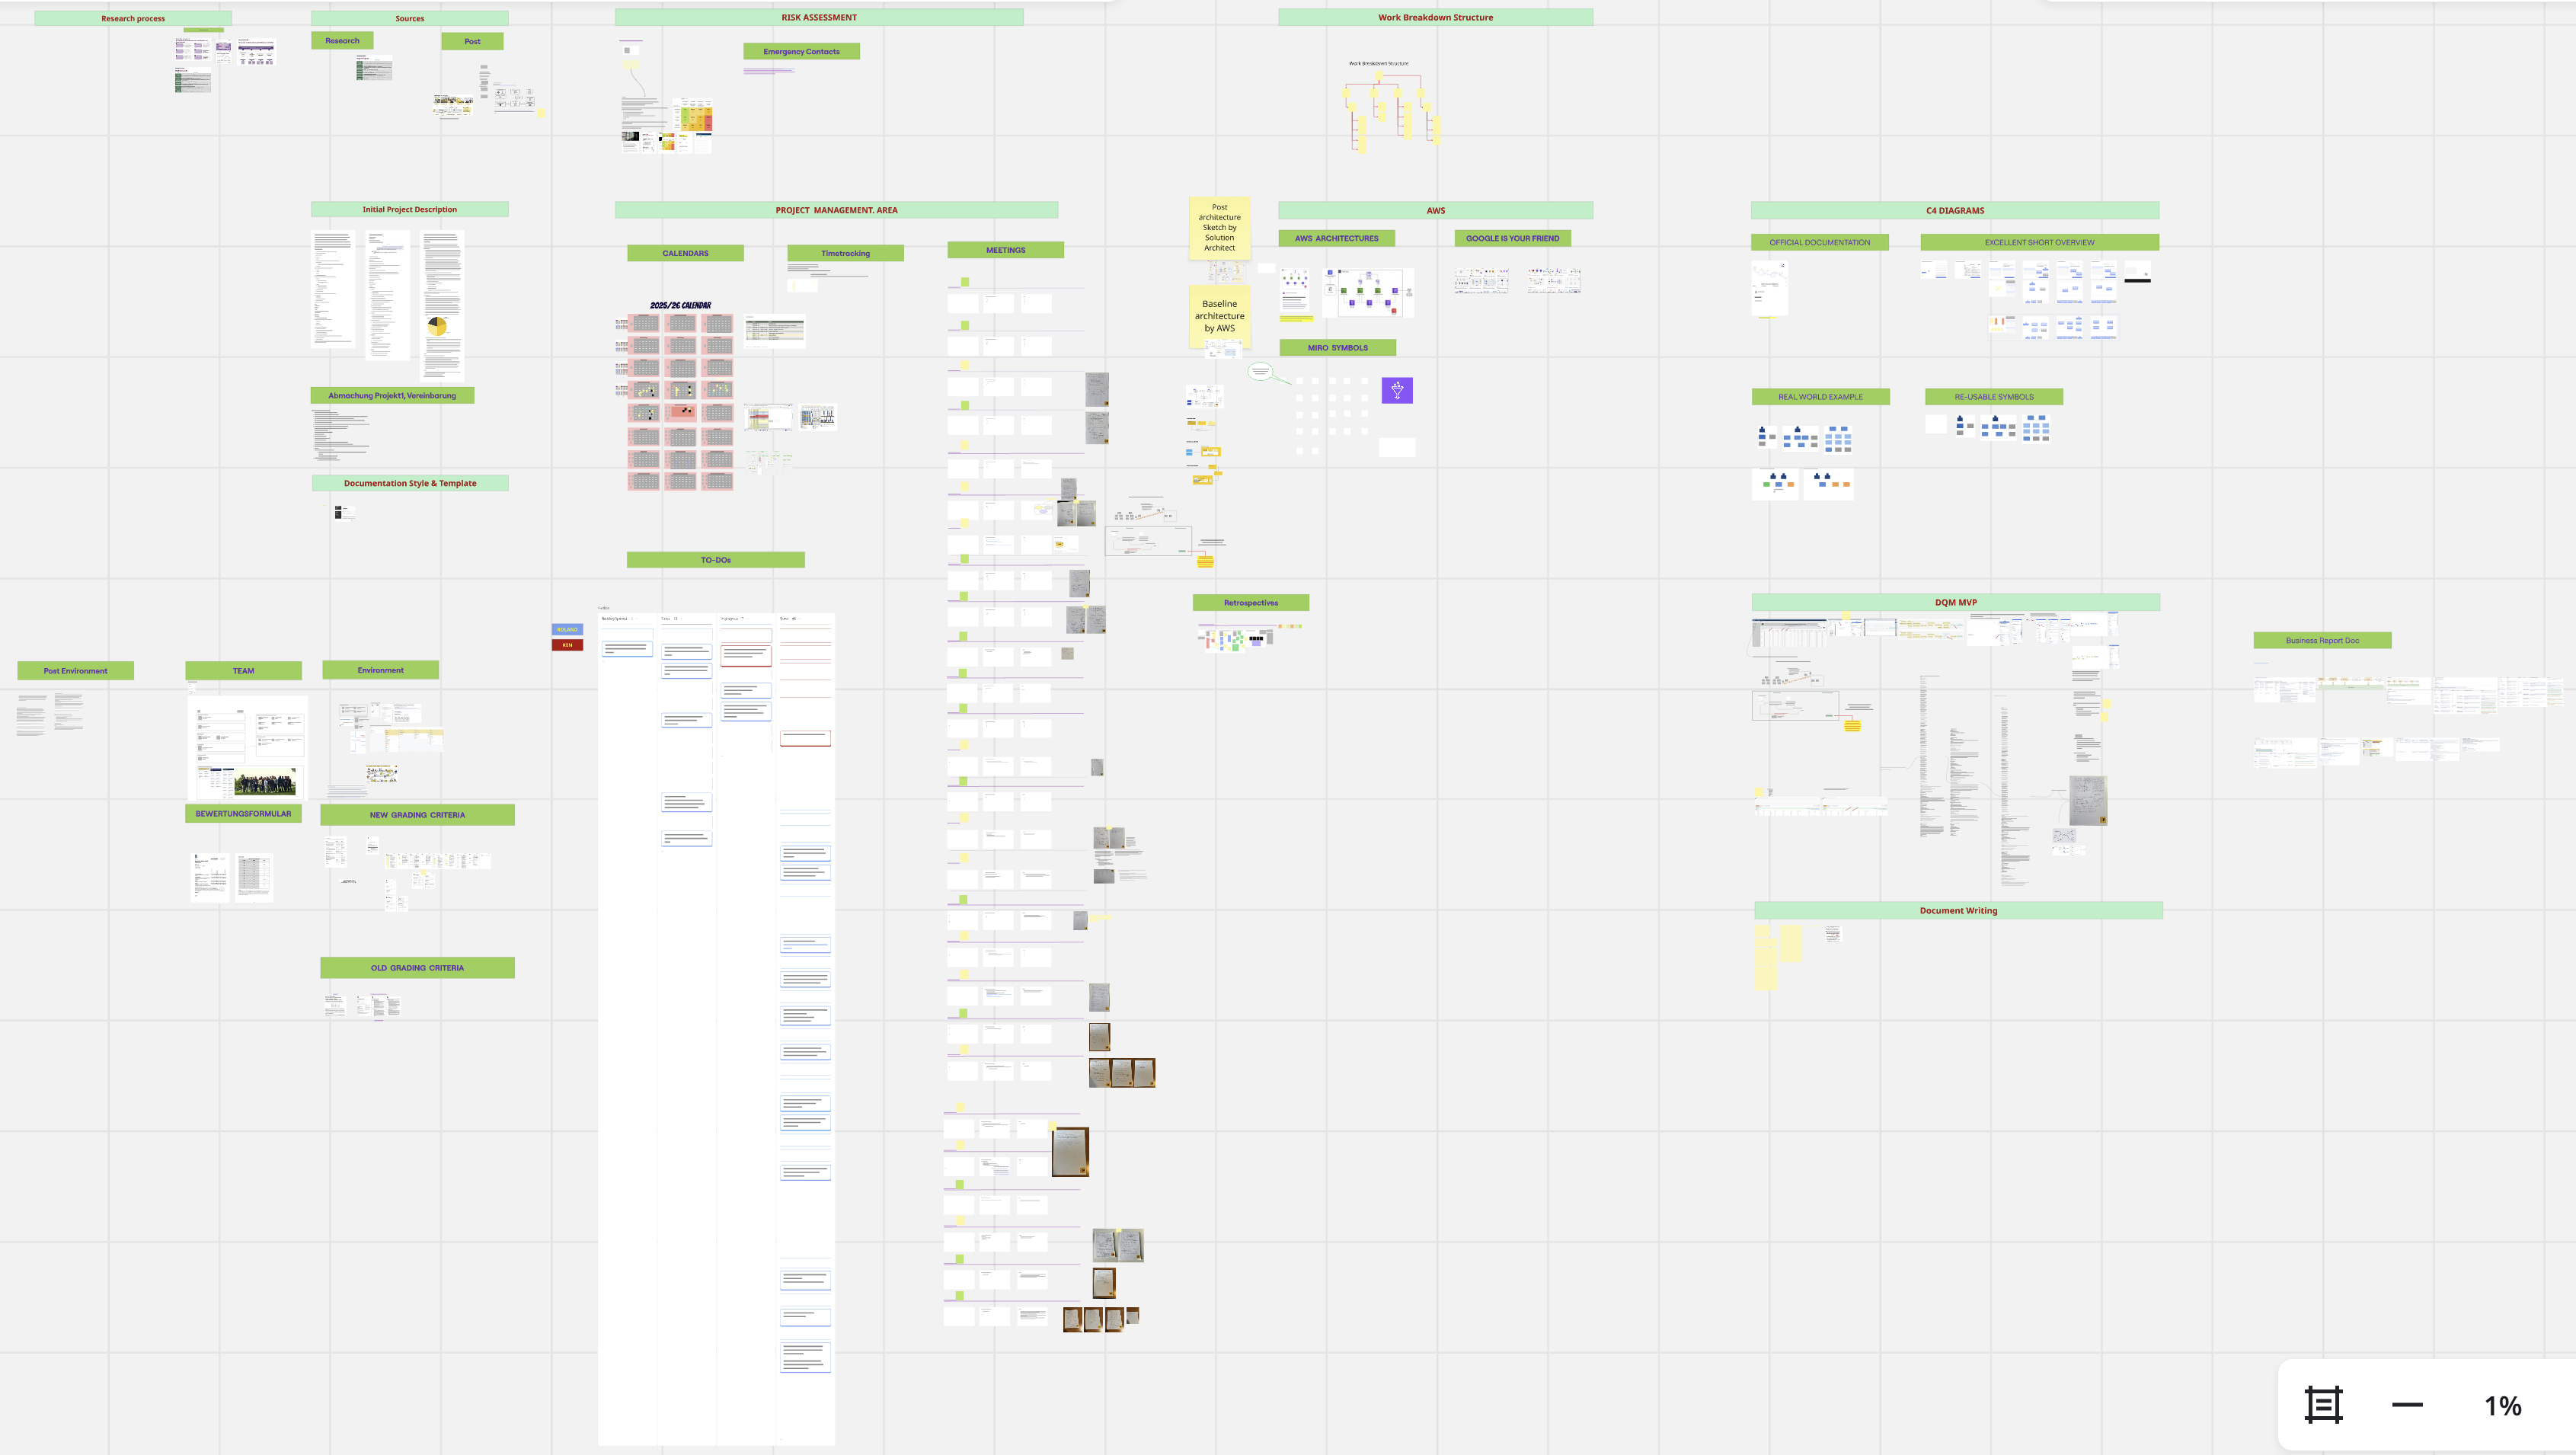
\includegraphics[width=0.8\textwidth]{./content/img/MiroBoard_23-12-2025.png}
    \caption{Miro board documentation, view of 23.12.2025}
    \label{fig:miro_final_board_twentythird_december}
\end{figure}

\subsubsection*{Miro calendar}
The calendar in Miro was primarily used to schedule the milestones. These are shown with green tiles on the corresponding dates, including their number and milestone title. Jour Fixe meetings are marked in yellow whenever they occurred, including adjustments in cases of unavailability. Actual unavailabilities at scheduled Jour Fixe meetings and other times are documented in black. Finally, holidays are marked in teal. In the case of this project, this applied only to the Christmas and New Year holiday period.

\begin{figure}[H]
    \centering
    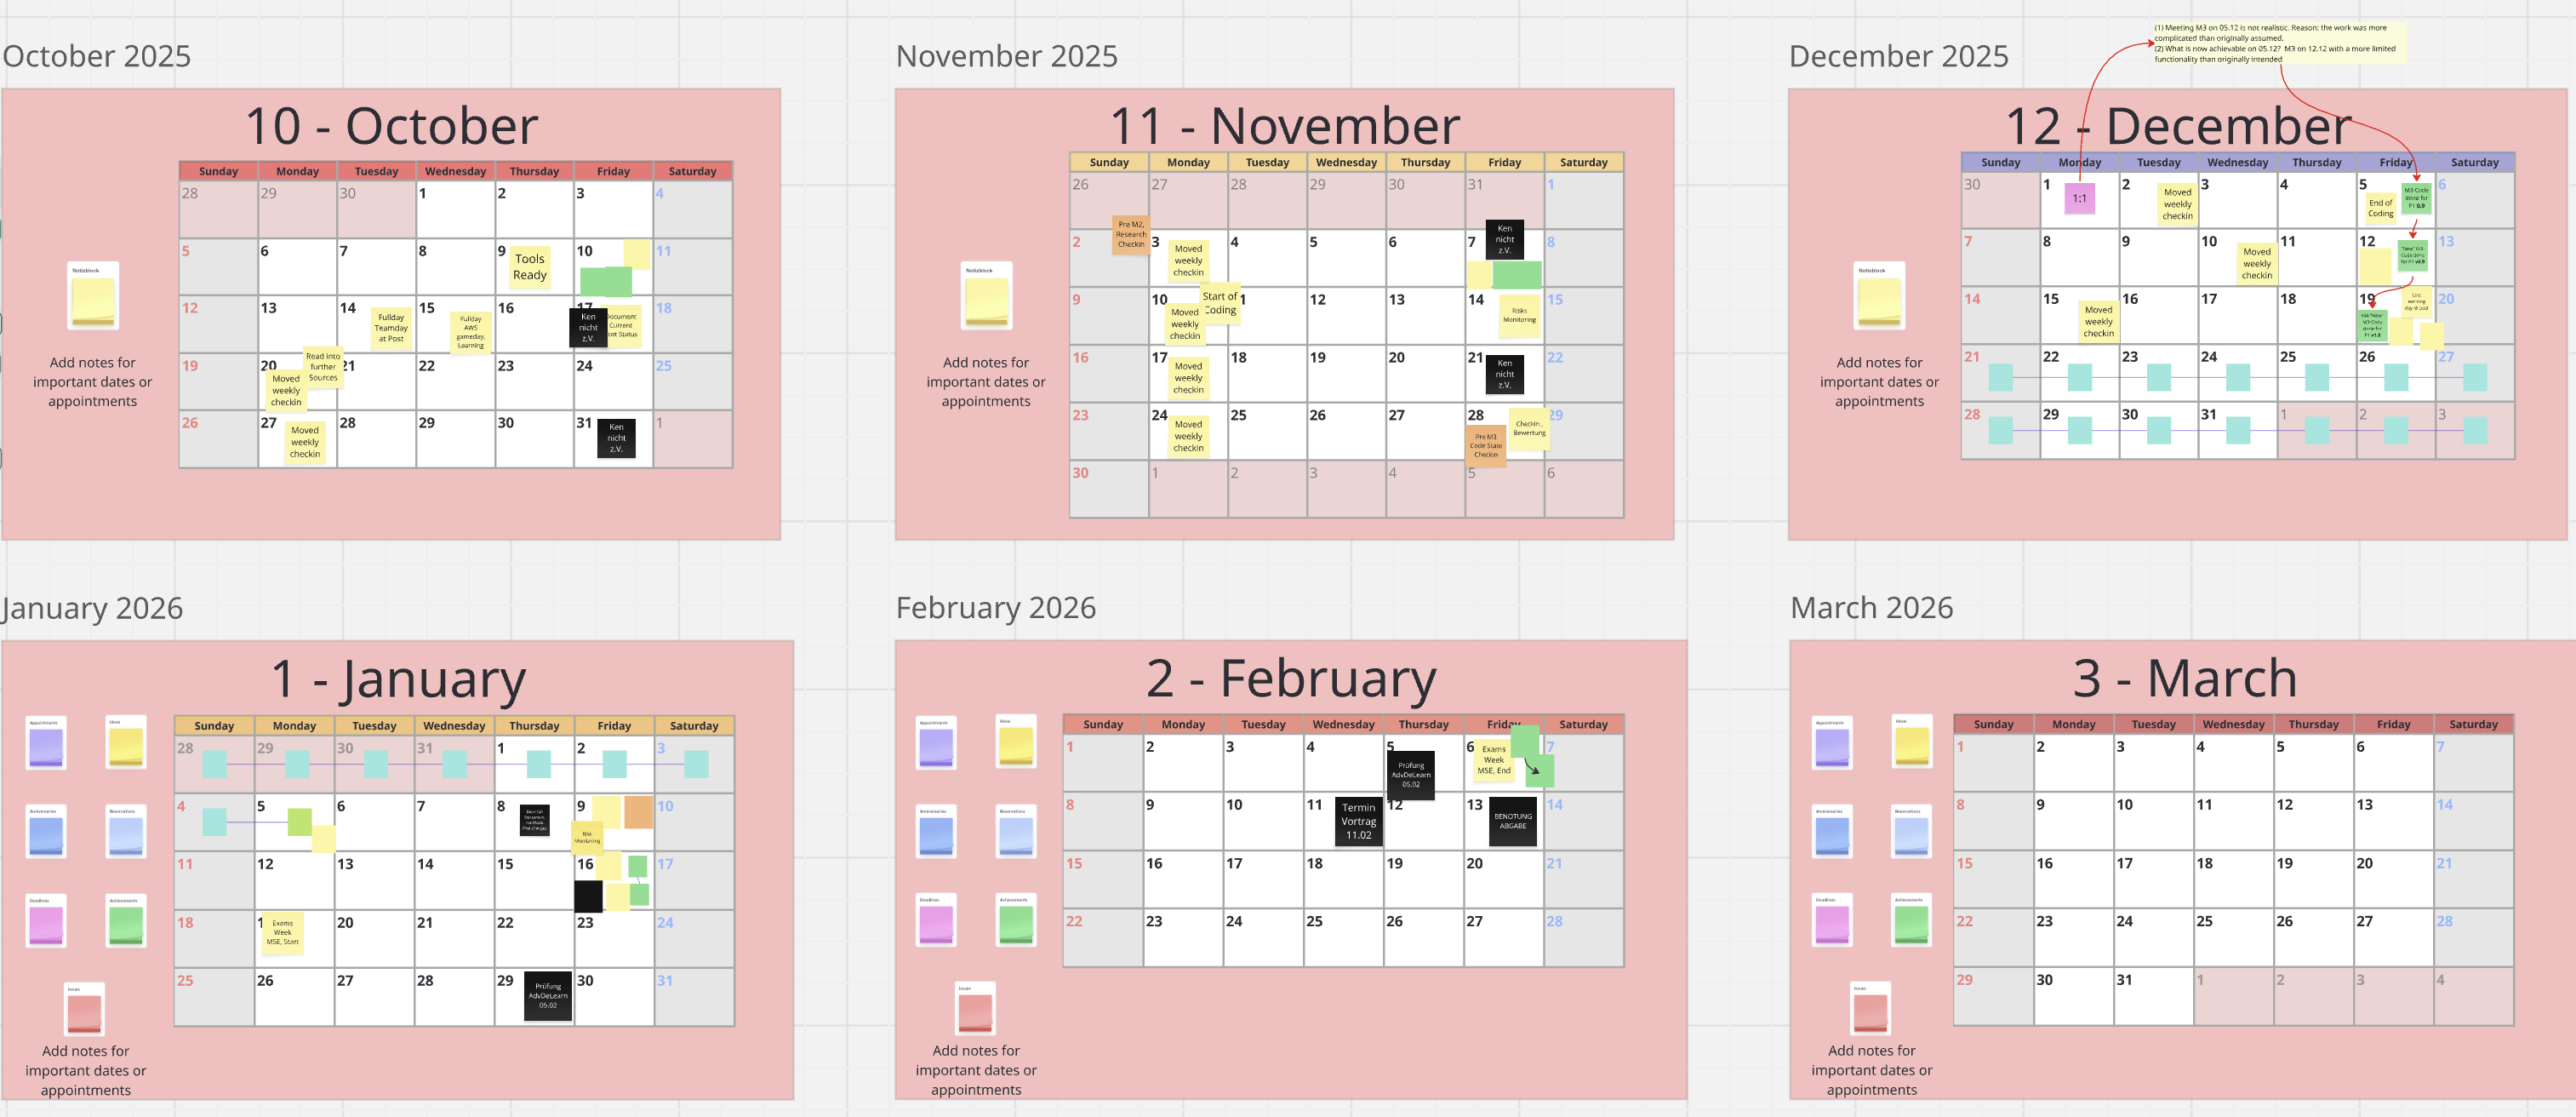
\includegraphics[width=0.8\textwidth]{./content/img/MiroBoard_Calendar.png}
    \caption{Miro board calendar used for coordination and tracking of milestones and related events}
    \label{fig:miro_board_calendar}
\end{figure}

\subsubsection*{Meetings documentation}
The meetings are documented using a layout with three sections, including a coloured tag at the top in yellow for Swiss Post meetings and green for academic ones. From left to right, these sections are structured as follows. First, the meeting points to be discussed are listed; these are copied from the Outlook invitations. Second, the topics addressed are summarised, mostly after the meeting. Third, the to-do block describes any actions that arose during the meeting. Not every meeting includes all sections. Furthermore, meetings are often documented using handwritten minutes. These are uploaded to the right of the meeting blocks without further refinement and serve as references.

\begin{figure}[H]
    \centering
    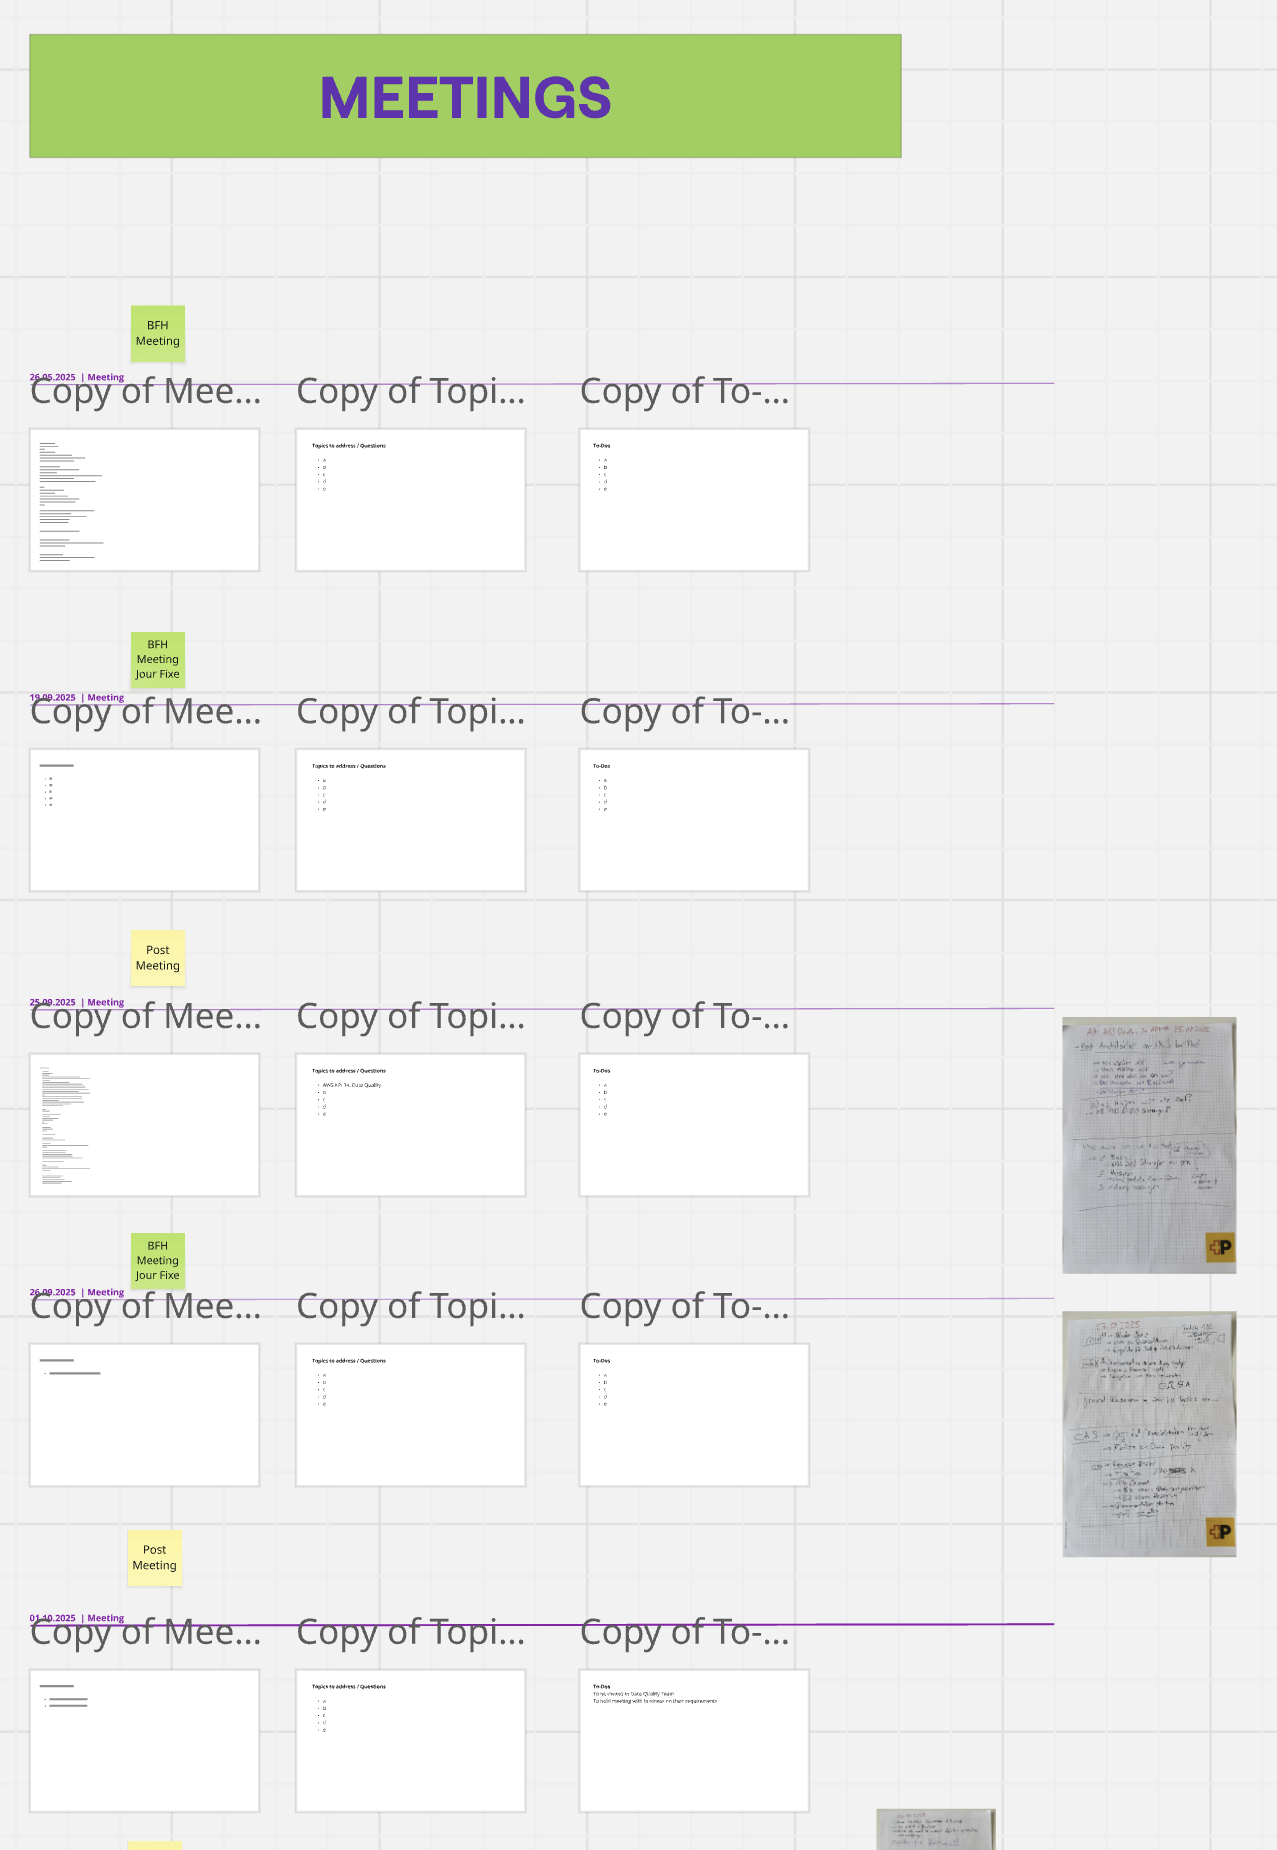
\includegraphics[width=0.8\textwidth]{./content/img/MiroBoard_Meetings.png}
    \caption{Miro board, tracking of meetings: when, who, what}
    \label{fig:miro_board_meetings}
\end{figure}

\subsubsection*{Documentation of the Implementation}
The implementation was first documented in Miro, as the rapid creation of screenshots did not disturb the flow of information gathering. In the following figure, the information-gathering process can be seen, starting from the top left, moving to the right, and then restarting from the left. First, screenshots of the SAC report are shown, followed by navigation towards DSP. Further details on the tools are described in the Implementation chapter.

\begin{figure}[H]
    \centering
    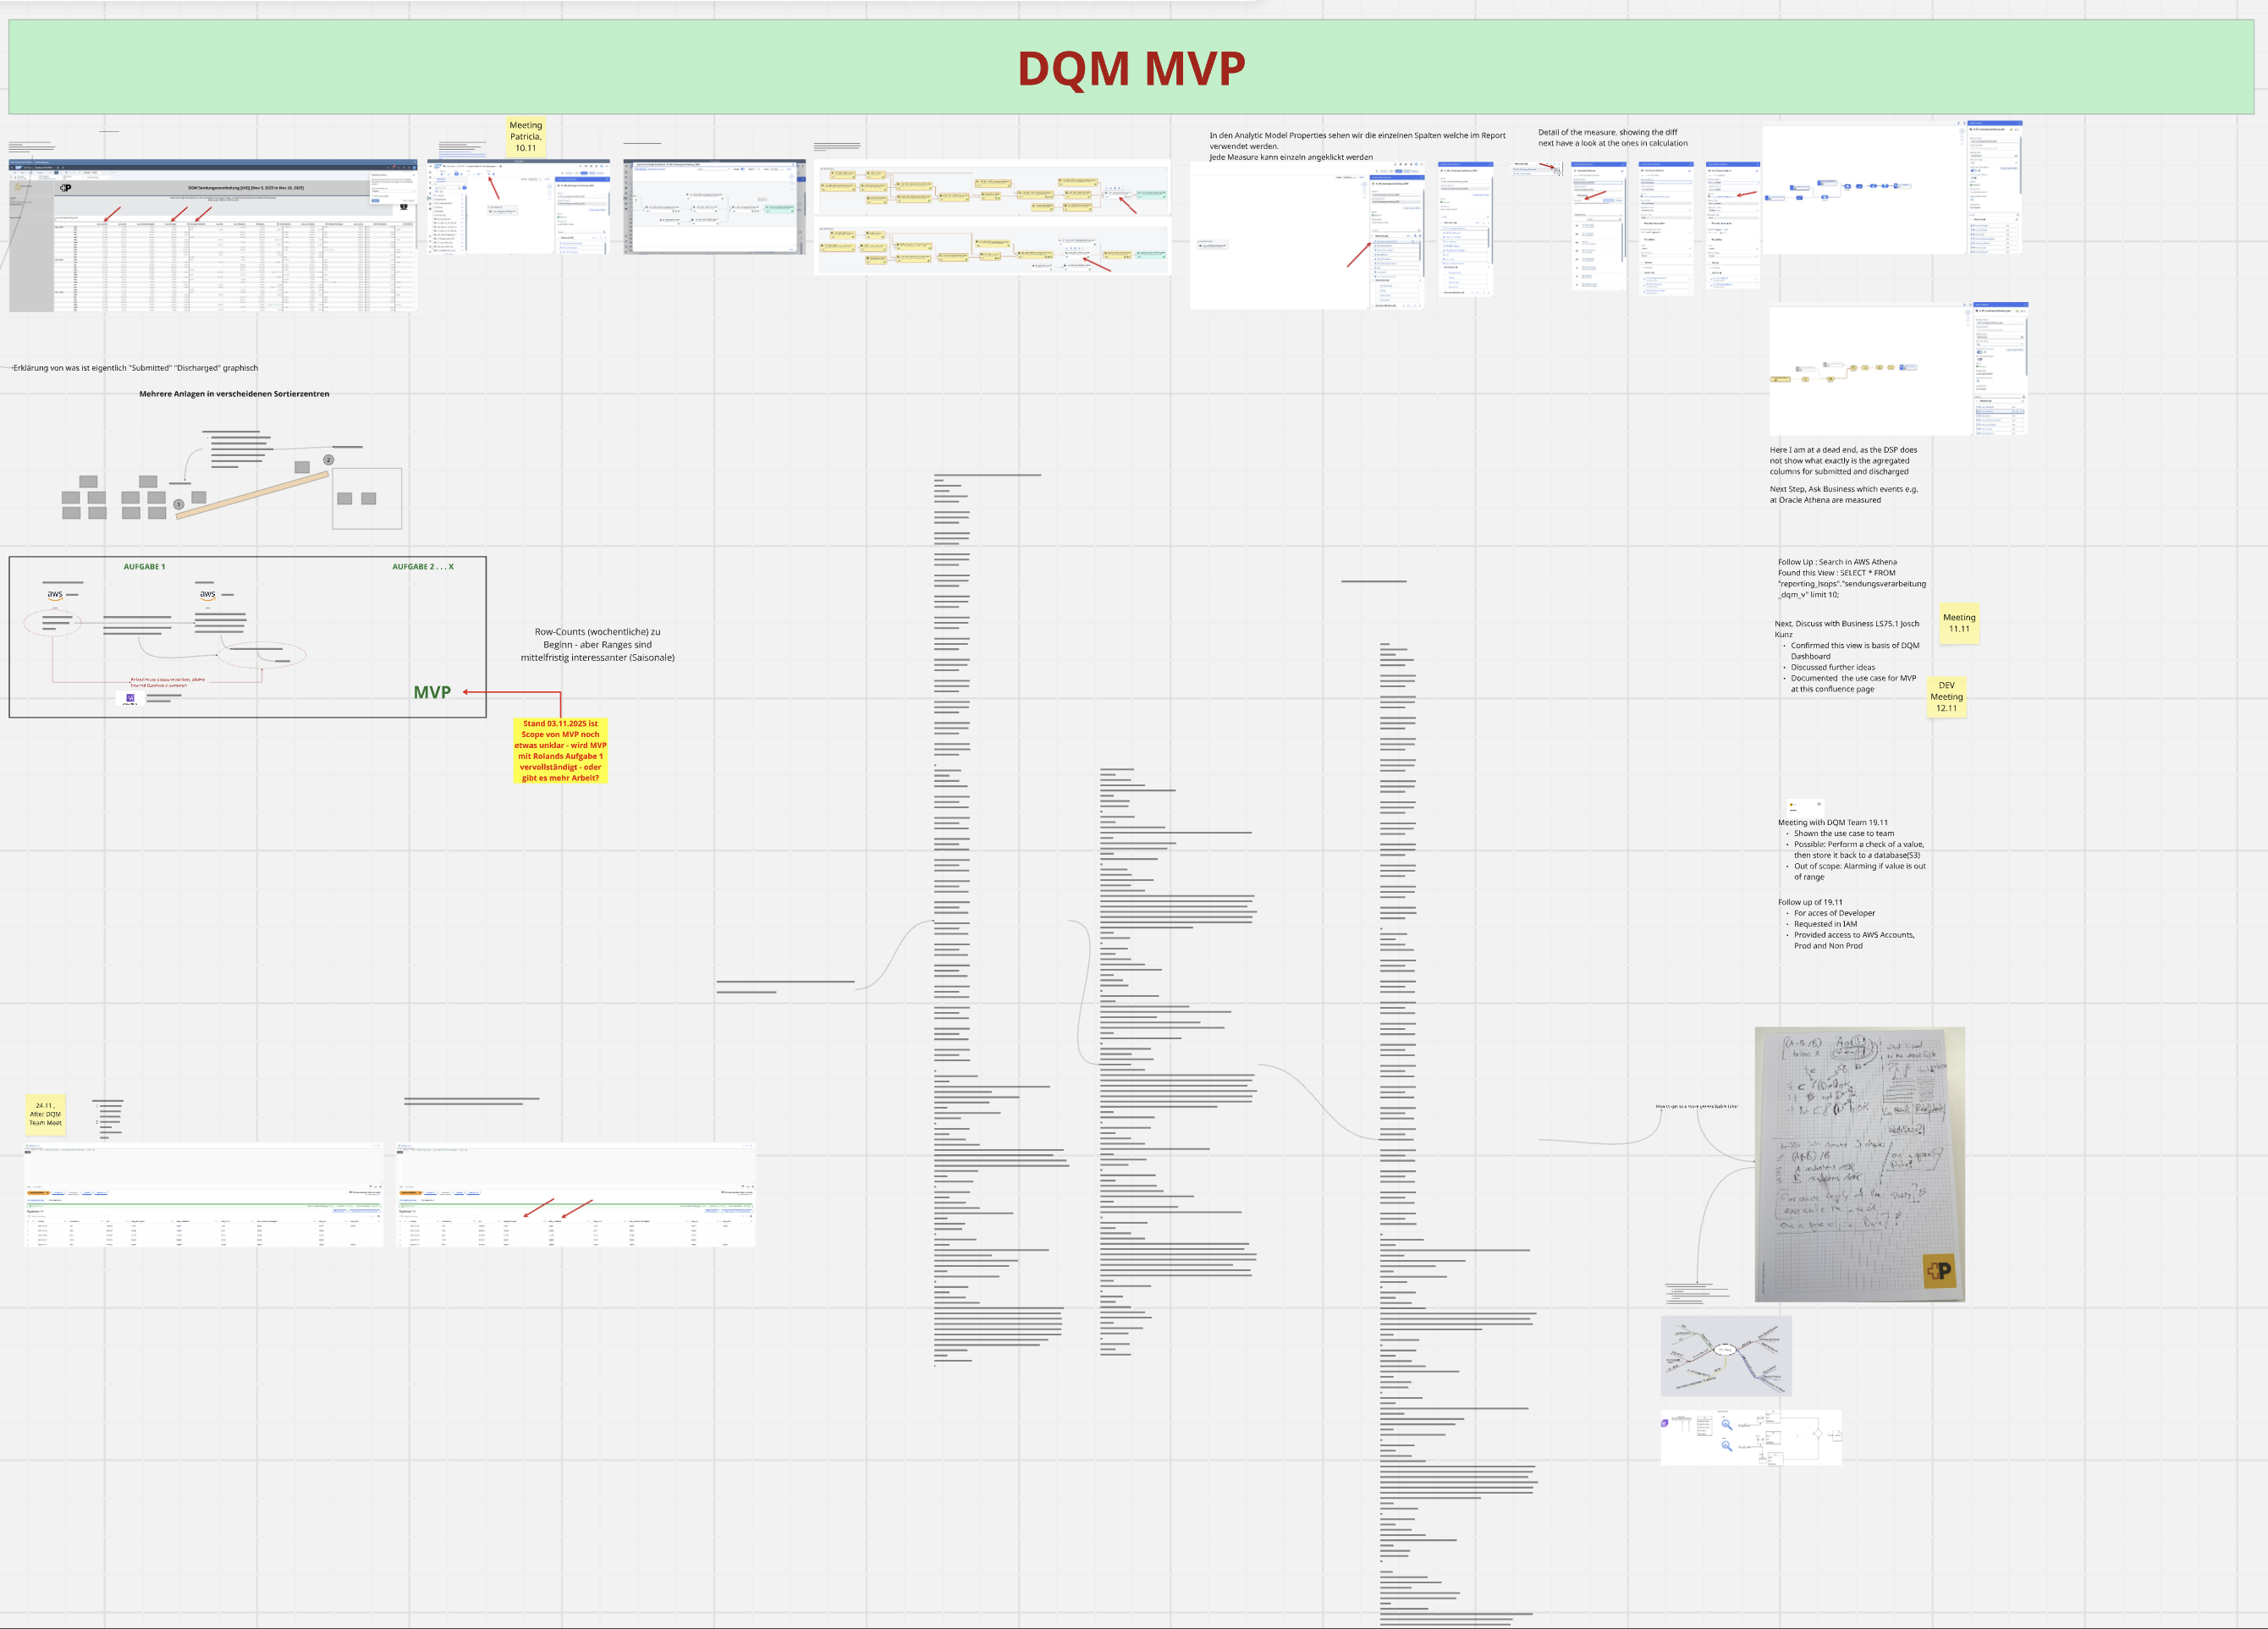
\includegraphics[width=0.8\textwidth]{./content/img/MiroBoard_Implementation.png}
    \caption{Miro board usage for quick documentation during implementation}
    \label{fig:miro_board_implementation}
\end{figure}


\subsection*{Jira and Confluence}

Jira (mainly for issue tracking) and Confluence (mainly for documentation) are both tools provided by Atlassian and are therefore well integrated with each other. The tools are installed on-premises, which limits sharing possibilities outside the Swiss Post network. They are used by the three Swiss Post teams presented in the Teams section. The project team also used Confluence when research results had to be presented as a first use case. While Jira is used for the short-term management of Scrum artefacts, Confluence is used for long-term documentation. An example of such long-term documentation is shown in the following screenshot, illustrating the documentation of a data lineage.

\begin{figure}[H]
    \centering
    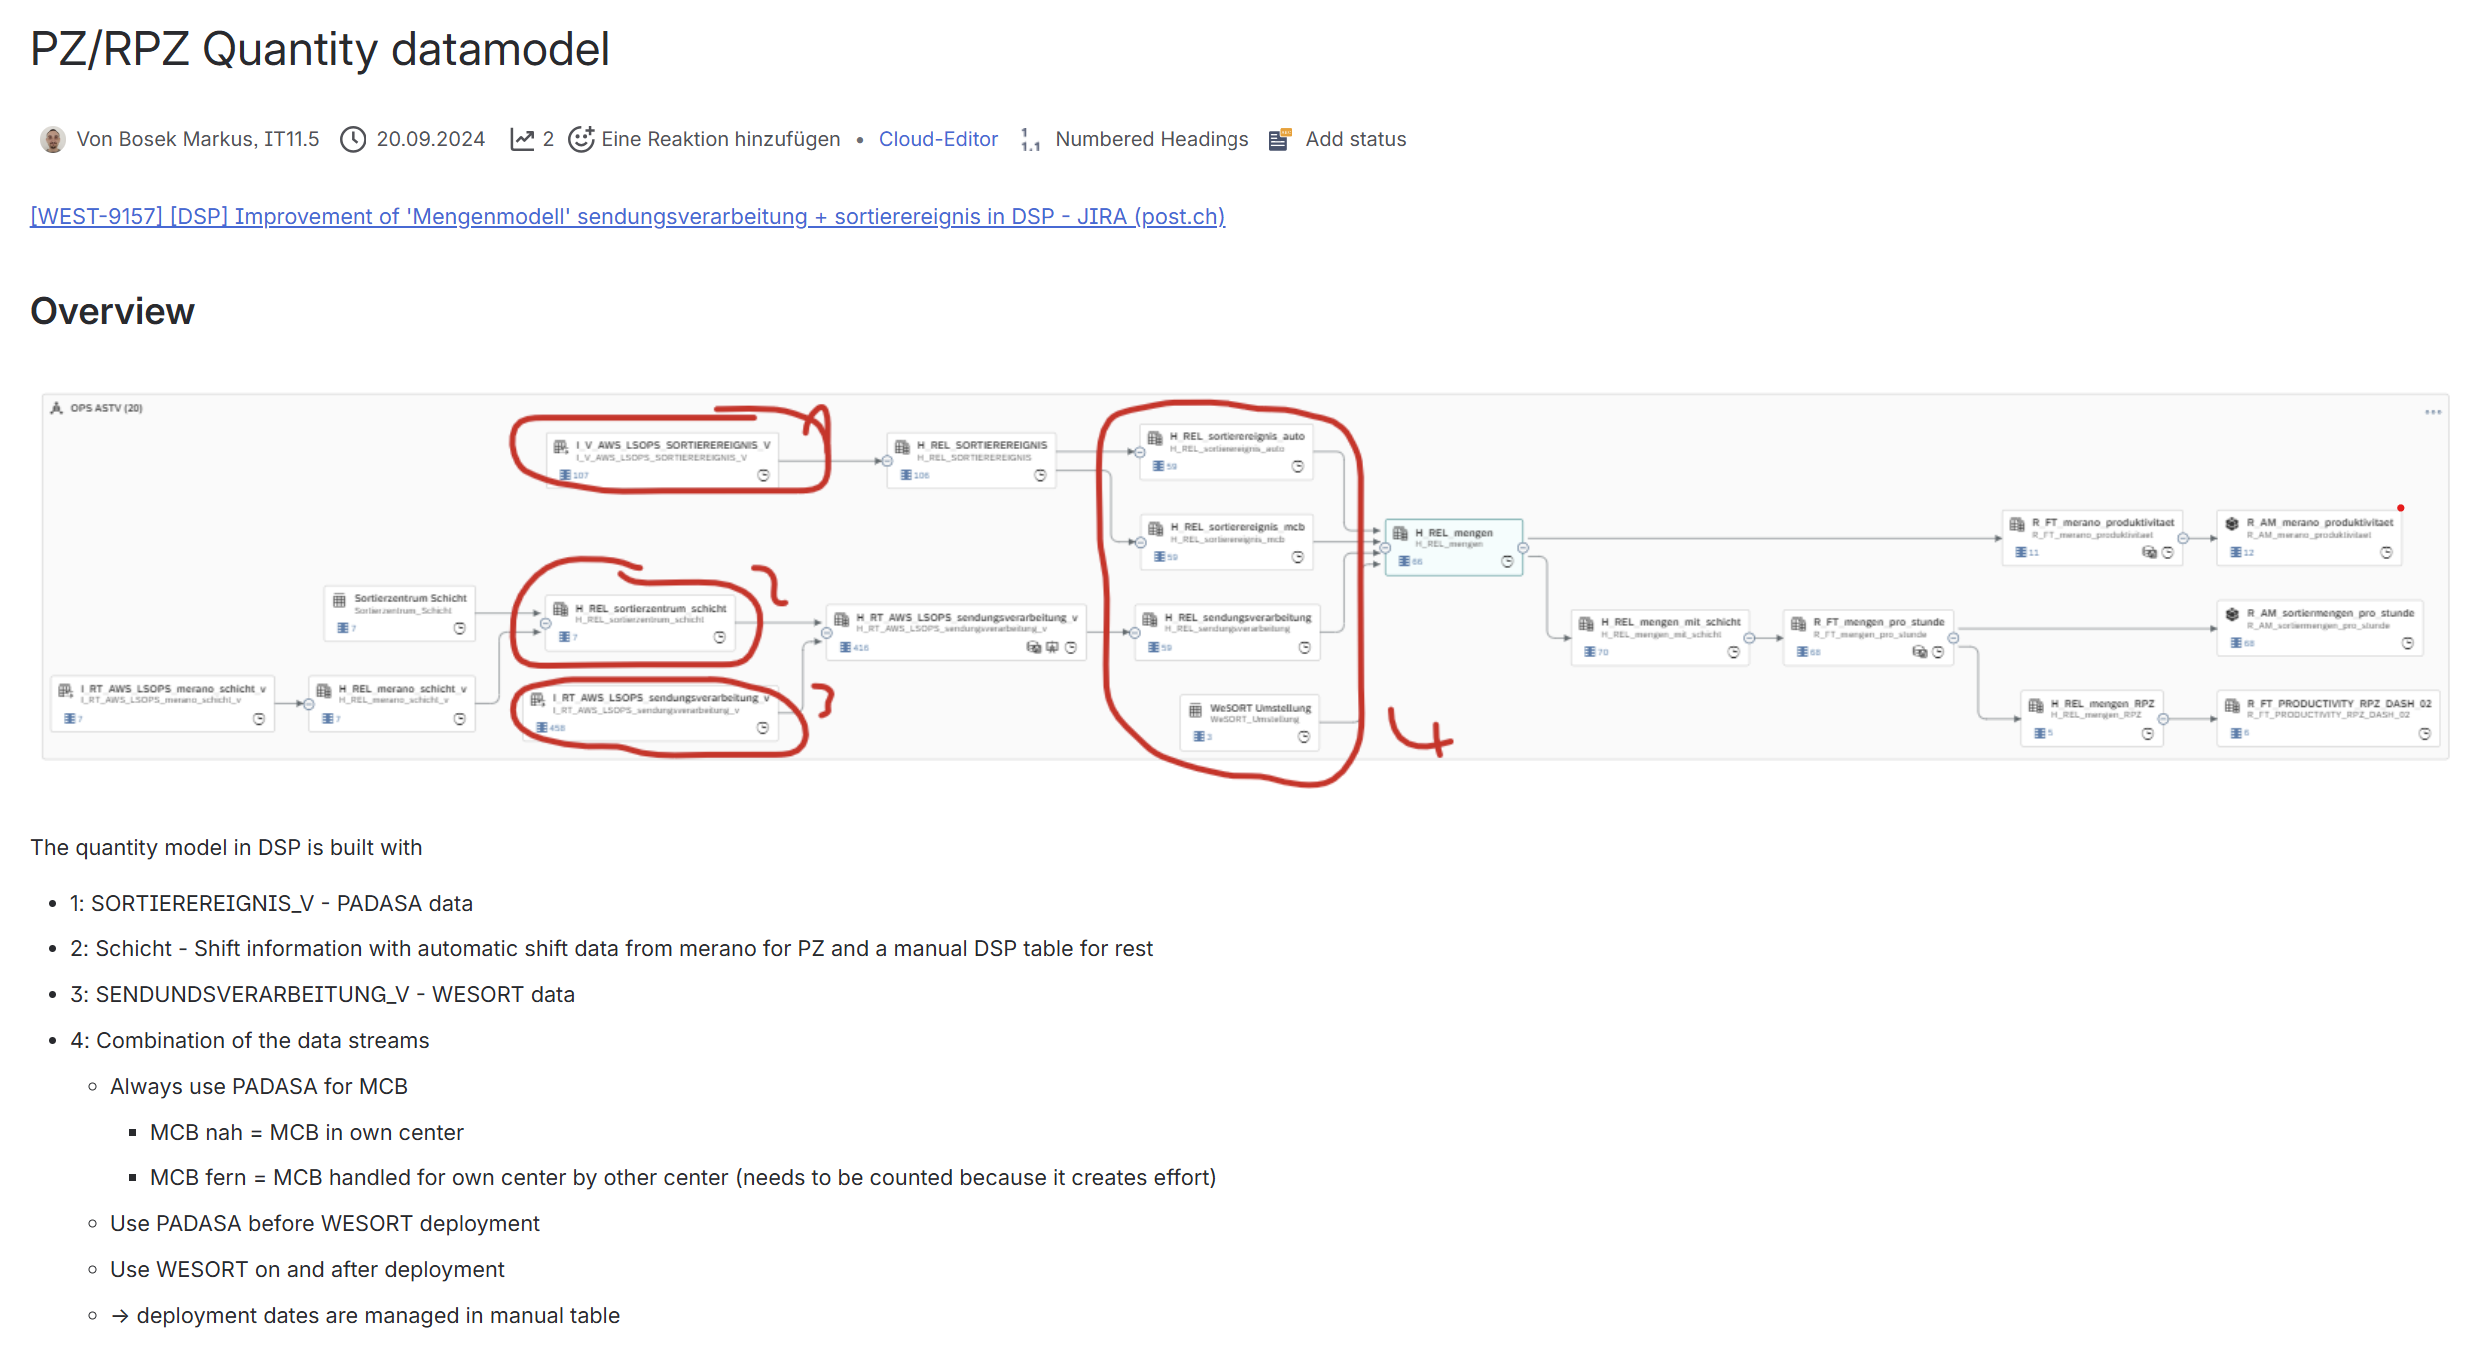
\includegraphics[width=0.95\textwidth]{./content/img/ProjectManagement/Confluence_usage_longtime_documentation.png}
    \caption{Example of project documentation in Confluence used to record architectural decisions and their rationale for future reference}
    \label{fig:confluence_architecture_documentation}
\end{figure}

\subsection*{Microsoft Teams and Microsoft Outlook}
MS Teams and MS Outlook are used by both the academic and Swiss Post teams. They are organisational standards at Swiss Post and are not optional. The same applies to the academic context. Both tools serve to support focused long-term (MS Outlook) and short-term (MS Teams) communication.

\subsection*{Shared chat}
For the academic team, the chat was used for short-term communication. However, a challenge arose due to the involvement of two distinct organisations, BFH and the Swiss Post. In order to keep communication between Swiss Post accounts and BFH accounts in one place, a chat with three users was required. In this context, the cross-organisational capabilities of MS Teams proved useful. After the Swiss Post account was invited to participate in the project team, it was able to communicate directly with BFH accounts. A sample of the communication involving three accounts is shown below.

\begin{figure}[H]
    \centering
    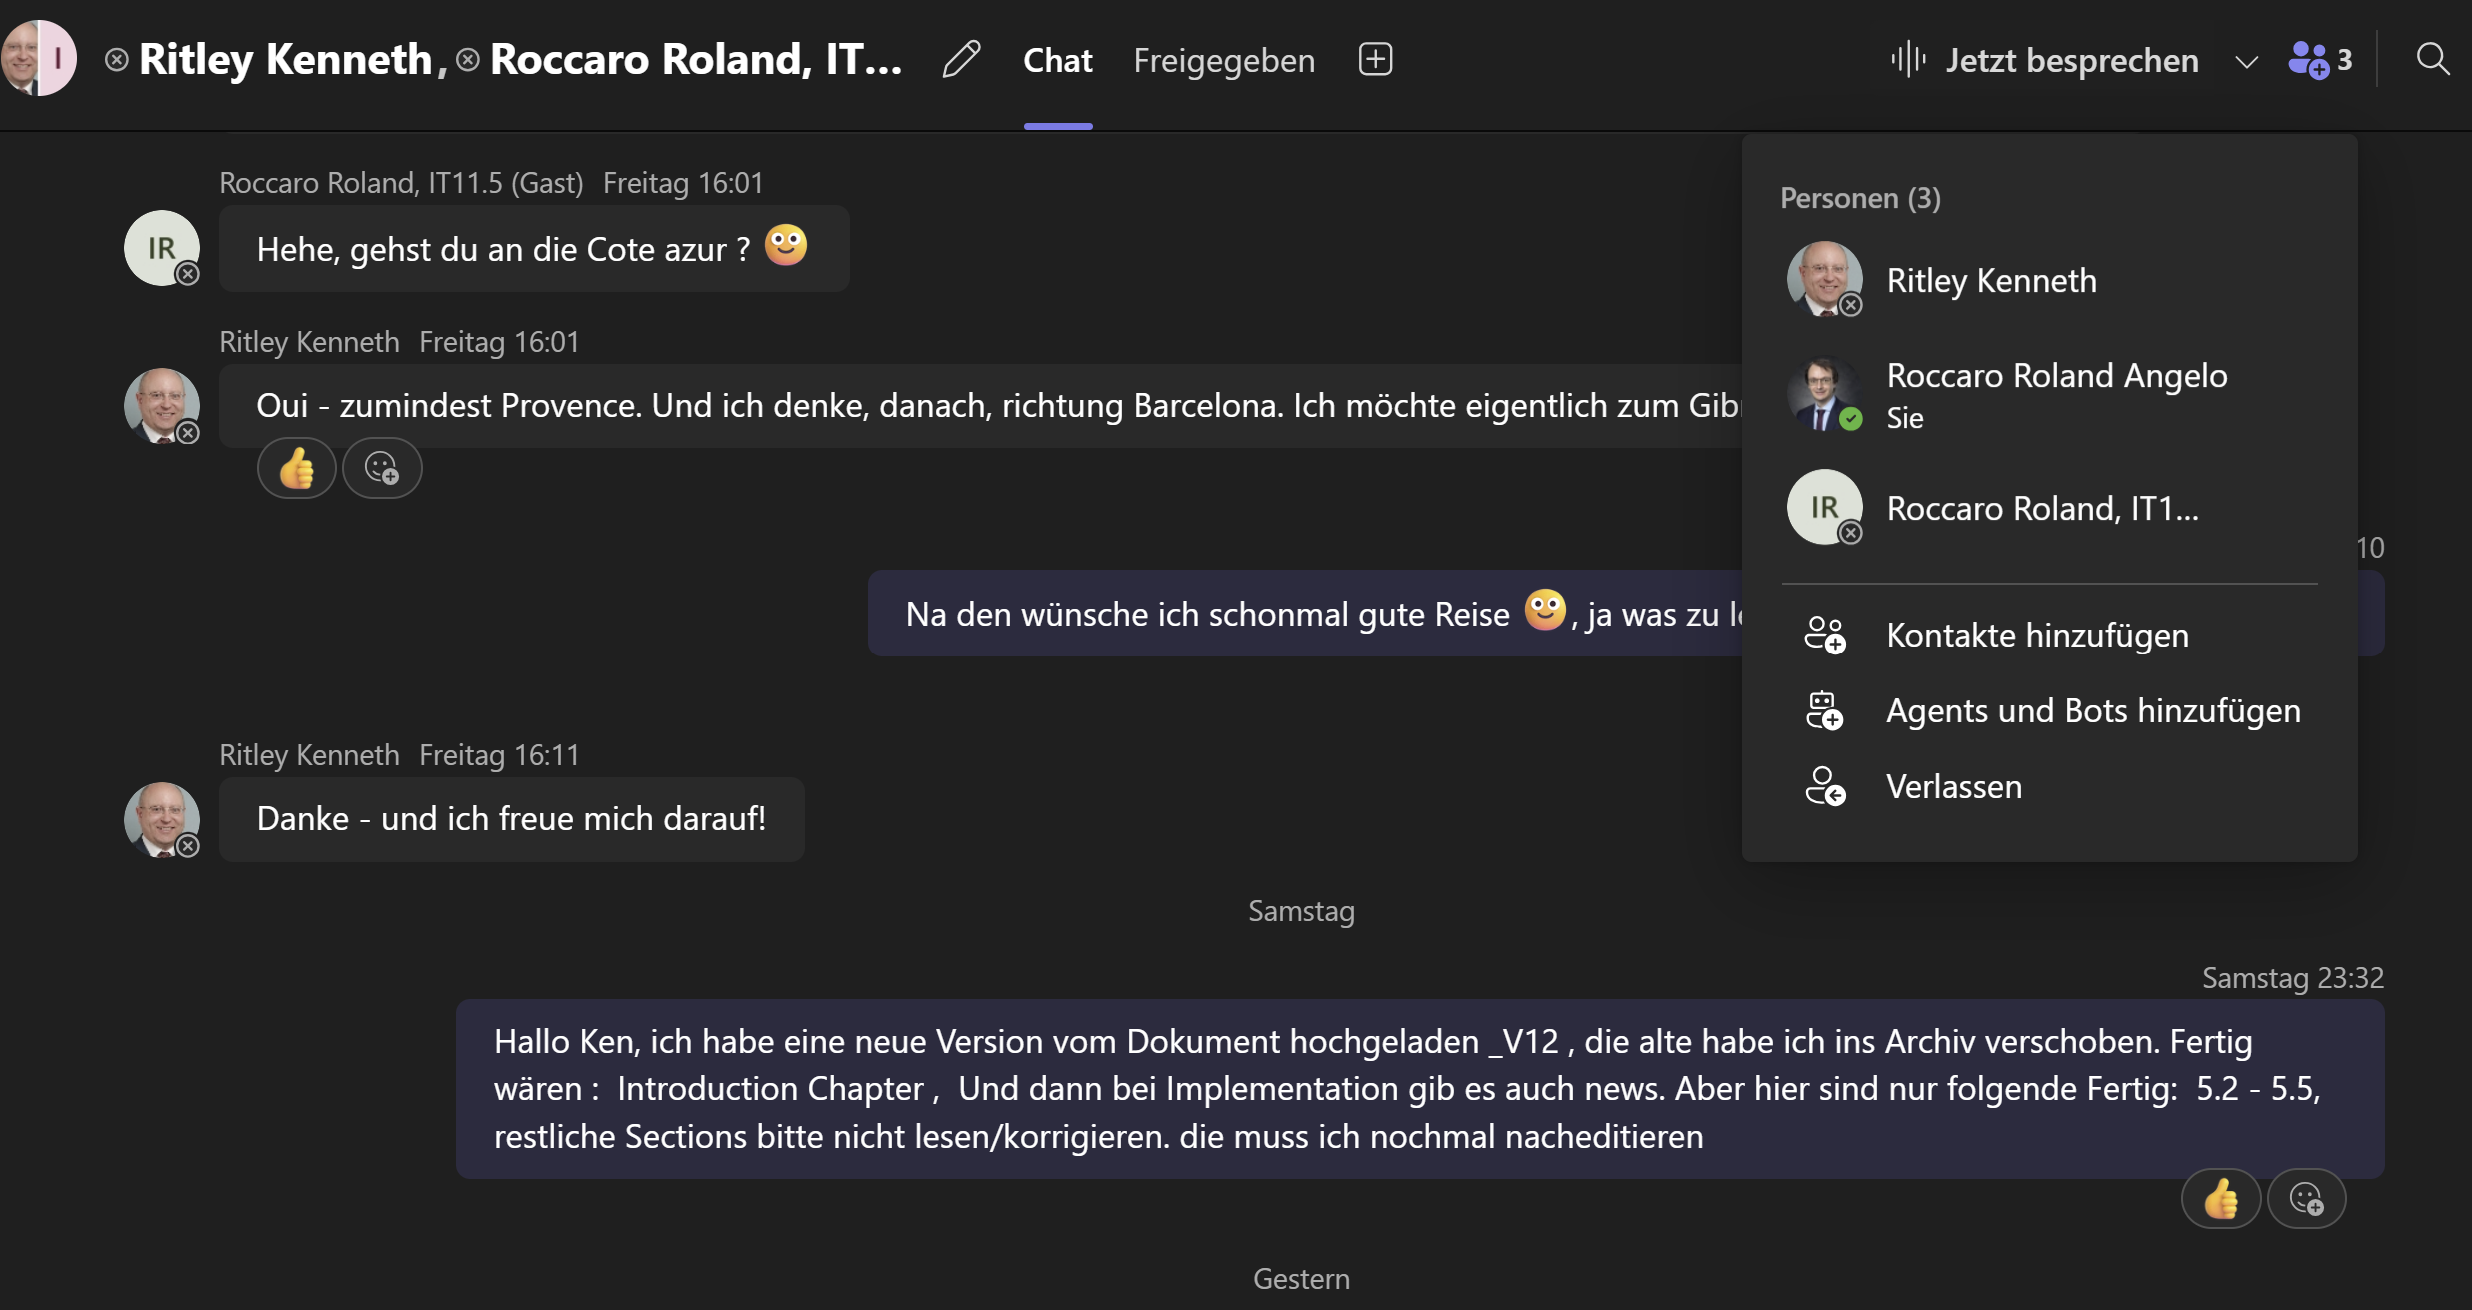
\includegraphics[width=0.8\textwidth]{./content/img/ProjectManagement/ProjMgmt_Teams_Chat.png}
    \caption{Shared chat using Teams}
    \label{fig:teams_shared_chat}
\end{figure}

A second important application of MS Teams is a document management system. This includes source documents, document versions, and related materials. All relevant documents are stored within this structure, which is designed to grow as needed.

\begin{figure}[H]
    \centering
    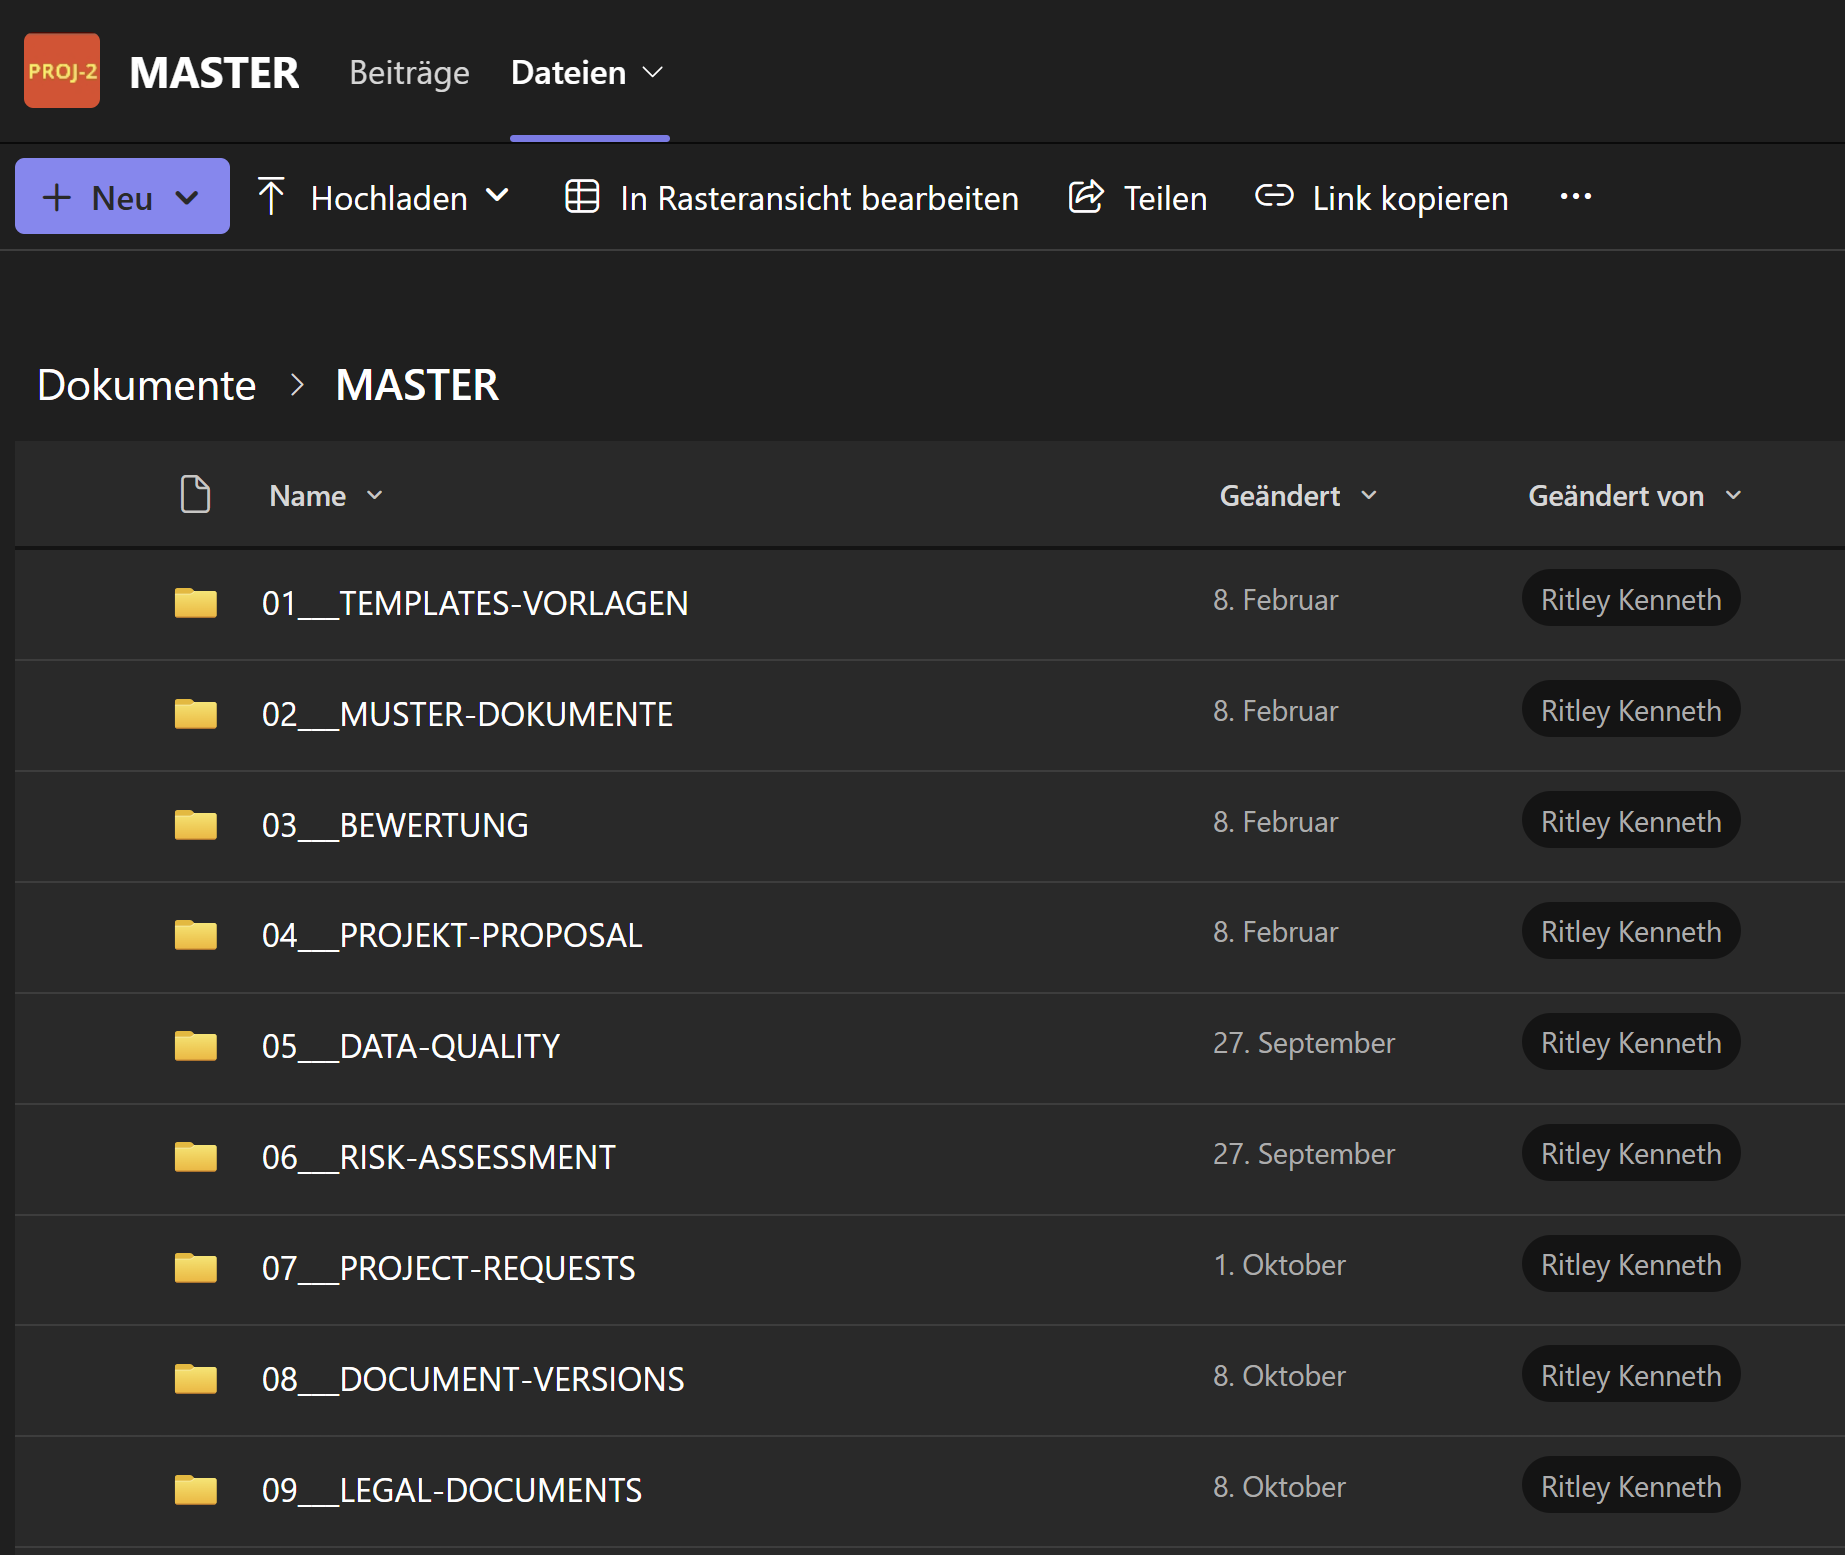
\includegraphics[width=0.8\textwidth]{./content/img/ProjectManagement/ProjMgmt_Teams_Documents.png}
    \caption{Project document store used with Teams}
    \label{fig:teams_document_store}
\end{figure}

\subsection*{LaTeX}
LaTeX was the tool chosen for the main writing process by the academic team. The primary reason for selecting this tool was the consistency of the document structure. It allows changes to be made in a large document without the document becoming unstable. The tool was specifically selected for this higher consistency compared to Word. The fact that the creation of some stylistic elements takes more time than with a \gls{WYSIWYG} editor such as Word was accepted, particularly as design was valued lower than document content. Finally, the consistency of being able to reference text sections within the document and the ability to automatically generate lists of figures and tables were seen as additional benefits. Furthermore, the automatic glossary and citation features using Biber were considered advantages for which the slower writing process without a WYSIWYG editor was accepted. Due to the learning effort involved in using \LaTeX, the following badge was earned during the course of the research.

\begin{figure}[H]
    \centering
    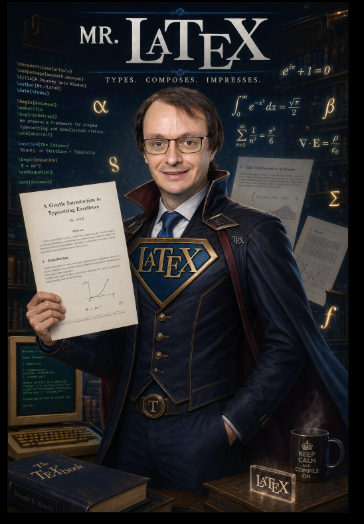
\includegraphics[width=0.65\textwidth]{./content/img/ProjectManagement/RolandMasterOfLatex.png}
    \caption{Humorous illustration symbolising the extensive use of \LaTeX\ throughout the preparation of this report and the associated learning experience during the project.}
    \label{fig:latex_mastery}
\end{figure}

\subsection*{GitHub}
For maintaining version control of any created artifacts, the public GitHub was used with the private account of the academic team. It was mainly used as a repository. This Git distribution was chosen because it is free to use and already well known to the team, with all required accounts in place, so no additional adoption or learning effort was required before starting. GitHub was not only used to store the document and track its progress, but also to manage all required sources such as tables and images used in the document.

For the writing process, the use of GitHub as a backup mechanism was particularly important. As all sources are stored in GitHub, the project was safeguarded against hardware failures of the working device, which is one risk mitigation measure. Continuously committing and pushing changes made the progress of the writing process traceable and supported the iterative writing approach which was chosen. This proved useful when the document PDF could no longer be generated, as the last version that compiled without errors could be identified. Finally, storing the sources on GitHub allowed access from different devices, which was useful when transferring materials such as screenshots from the work device to the study device.

\subsection*{ChatGPT}
LLMs are now an indispensable part of work. To note how ChatGPT was used in this project, it was given the following prompt:
\begin{quote}
Hi ChatGPT, please look at the other chats I have with you and tell me in which ways you supported me during my academic project over the past months since September 2025. Please create a subsection for my scientific work which I can reference.
\end{quote}

The following subsection was completely AI generated content by ChatGPT, without further editing.
{\itshape
\subsubsection*{ChatGPT}

To document the support provided by ChatGPT, a summary of the assistance received during the academic project was generated directly by the tool itself:
The request asked ChatGPT to review prior interactions and describe the ways in which it supported the academic project over the past months since September 2025. The resulting subsection is intended for inclusion in the scientific work and can be referenced accordingly \cite{chatgpt_ai_assistance_2025}.



The following subsection is entirely AI-generated content produced by ChatGPT, without further editing  \cite{chatgpt_ai_assistance_2025}.

\subsubsection*{Use of AI Assistance in the Research Process}

Since September 2025, the author has used the AI language model \emph{ChatGPT} as a supportive tool during the development of this academic project. The assistance provided did not replace independent scientific work but complemented it in the following ways:

\paragraph{Conceptual Clarification and Structuring}
ChatGPT was used to support the clarification of complex theoretical concepts, the refinement of research questions, and the improvement of the logical structure of arguments. This included exploring alternative formulations, identifying conceptual gaps, and supporting the organization of sections and chapters.

\paragraph{Language and Academic Writing Support}
The tool assisted in improving the clarity, coherence, and academic tone of the manuscript. This included rephrasing passages for precision, adjusting wording to meet scientific standards, and supporting grammatical accuracy and stylistic consistency across the text.

\paragraph{Methodological Reflection}
ChatGPT supported reflective discussions regarding methodological choices, including the articulation of research design, limitations, and the justification of selected approaches. All methodological decisions, interpretations, and final formulations remained the sole responsibility of the author.

\paragraph{Iterative Feedback and Revision}
Throughout the research process, ChatGPT was used as an iterative feedback instrument to review draft sections, explore alternative explanations, and identify areas requiring further refinement or clarification.

\paragraph{Ethical and Responsible Use}
ChatGPT did not generate original empirical data, conduct analyses independently, or make autonomous scientific claims. All AI-generated content was critically evaluated, revised, and integrated by the author in accordance with principles of academic integrity and responsible research practice.
}
\section{Timetracking}
As part of the need for transparency and the ability to review the efforts committed to this project, time tracking was performed from the start to the end of this documentation. The tracked time was recorded in two separate ways. Work efforts carried out within Swiss Post were captured directly from the Swiss Post \gls{MIAR} system, noting only the time spent per day without further details on the specific tasks performed. This information was saved in an Excel file and marked as work effort.

Second, academic efforts committed to the project outside the Swiss Post context were recorded directly in an Excel file. For each work block, a separate entry was created. A block represents continuous work on project-related tasks, including short breaks; however, longer breaks, such as lunch, resulted in a new block being created. Excel was used because the Office suite was already in use for other purposes, and the information did not justify storage in a more complex database such as MariaDB. The tracked time is not intended for billing or performance measurement, nor is it used to assess milestone performance.


\section{Risk management}
\label{ProjMgmtRisk}
In this section, the approach taken to risk management is described. Risk management is essential to the success of any project, as it enables planning for and potentially preventing dangers that may occur during its course. When such risks are not handled, they can endanger the progress of the project. The risk management process consists of several steps \cite{RiskmgmtWikipedia}. First, the risks are identified and classified as to their nature. Next, they are weighted according to how they might impact this project; this includes a consideration of the probability that the risks may arise, and the level of damage that may occur. After this, the specific handling of each risk is defined; these are the concrete measures that are taken to lower how the risk may impact the project. Finally, ongoing monitoring and review of the risks is carried out on a regular basis throughout the project.

\subsection*{Risk identification and classification}

The identification of risks has been carried out for this project, following an extensive brainstorming approach. Each risk has been grouped into a category (e.g. goal, time and organization, etc.), and each risk has been classified according to the likelihood of is occurance and severity it would cause to the project. Both criteria are evaluated based on the project team’s \gls{riskappetite} and ranked according to the following definitions.

\begin{itemize}
    \item \textbf{Likelihood:} What is the expected likelihood of a risk coming into effect
    \begin{itemize}
        \item \textbf{1} Rare
        \item \textbf{2} Unlikely
        \item \textbf{3} Possible
        \item \textbf{4} Likely
        \item \textbf{5} Almost Certain
    \end{itemize}

    \item \textbf{Severity:} How severe are the consequences of the risk coming into effect
    \begin{itemize}
        \item \textbf{1} Insignificant
        \item \textbf{2} Minor
        \item \textbf{3} Moderate
        \item \textbf{4} Major
        \item \textbf{5} Severe
    \end{itemize}
\end{itemize}

The identified  risks, along with their likelihood and severity, are listed in Table \ref{tab:risks}.

\begin{longtable}{@{} C{1.1cm} L{3.2cm} L{8.1cm} C{1.6cm} C{1.6cm} @{}}
\caption{Project Risk Overview}\label{tab:risks}\\


\toprule
\textbf{No.} & \textbf{Group} & \textbf{Risk} & \textbf{Likelihood} & \textbf{Severity} \\
\midrule
\endfirsthead

\toprule
\textbf{No.} & \textbf{Group} & \textbf{Risk} & \textbf{Likelihood} & \textbf{Severity} \\
\midrule
\endhead

\midrule
\multicolumn{5}{r}{\small Continued on next page} \\
\endfoot

\bottomrule
\endlastfoot

1  & Goal & Unclear question & 2 & 2 \\
2  & Goal & Unclear goals & 2 & 3 \\
3  & Time and Organisation & Insufficient expertise & 4 & 2 \\
4  & Time and Organisation & Underestimated time/effort & 4 & 3 \\
5  & Time and Organisation & Other study projects & 3 & 3 \\
6  & Time and Organisation & Work projects & 4 & 3 \\
7  & Time and Organisation & Procrastination & 3 & 2 \\
8  & Human Resources & Unavailability of main project staff (e.g., due to illness) & 4 & 4 \\
9  & Human Resources & Unavailability of advisor (e.g., due to illness, accident, etc.) & 3 & 4 \\
10 & Tech and Infrastructure & Software Version/Library/Dependency & 4 & 3 \\
11 & Tech and Infrastructure & Hardware is damaged & 2 & 5 \\
12 & Data and Research & Data related & 4 & 3 \\
13 & Data and Research & Not reproducible work & 2 & 5 \\
14 & Ethical and Legal & Plagiarism or wrong citation & 2 & 5 \\
15 & Ethical and Legal & Copyright & 1 & 5 \\
16 & Communication and Cooperation & Bad communication with stakeholder or advisor & 2 & 4 \\
17 & Communication and Cooperation & Insufficient exchange with external partners & 1 & 5 \\
18 & Force Majeure & Unforeseen family crisis & 2 & 5 \\
19 & Force Majeure & General force majeure & 1 & 5 \\
\end{longtable}


\subsection*{Risk heat map}
After carrying out the initial identification and classification, it is not always easy to determine which risks require the most attention. To support this task, a Risk Heat Map is used, in which each risk is plotted in a two-dimensional matrix according to its likelihood and severity. This visualisation highlights the risks that pose the greatest threat to the project and should be considered for priority treatment. The colours in the Risk Heat Map \ref{tab:risks_sev_likely} correspond to these descriptions.


\begin{itemize}
    \item \textbf{Green} Low
    \item \textbf{Yellow} Medium
    \item \textbf{Orange} High
    \item \textbf{Red} Very High
\end{itemize}


\begin{table}[h]
\centering
\setlength{\tabcolsep}{3pt}
\renewcommand{\arraystretch}{1.6}
\label{tab:risks_sev_likely}
% 7 columns total: [1] merged "Severity" column + [2] row labels + [5] severity levels
\begin{tabular}{|C{1.3cm}|C{2.8cm}|*{5}{C{2.6cm}|}}

% --- Top black title row: span first two columns for title, last five for "Severity" header label ---

\hline
\rowcolor{black}
\multicolumn{2}{|c|}{\color{white}\bfseries Risk Matrix} &
\multicolumn{5}{c|}{\color{white}\bfseries Severity} \\
\hline

% merged first column (6 rows high)

\multirow{6}{*}{\cellcolor{white}{\color{black}\bfseries \rotatebox{90}{Severity}}}
  & \cellcolor{riskgrey}{}  % empty label cell
  & \cellcolor{riskgrey}\bfseries 1: Insignificant
  & \cellcolor{riskgrey}\bfseries 2: Minor
  & \cellcolor{riskgrey}\bfseries 3: Moderate
  & \cellcolor{riskgrey}\bfseries 4: Major
  & \cellcolor{riskgrey}\bfseries 5: Severe \\
\hline

% ---- Row 1 ----
& \cellcolor{riskgrey}\bfseries 5: Almost Certain
& \cellcolor{riskyellow}{\bfseries 15\; 17\; 19\;}
& \cellcolor{riskorange}{\bfseries 11\; 14\;}
& \cellcolor{riskred}{}
& \cellcolor{riskred}{}
& \cellcolor{riskred}{} \\
\hline

% ---- Row 2 ----
& \cellcolor{riskgrey}\bfseries 4: Likely
& \cellcolor{riskyellow}{\bfseries}
& \cellcolor{riskorange}{\bfseries 16}
& \cellcolor{riskorange}{\bfseries 9}
& \cellcolor{riskred}{\bfseries 8}
& \cellcolor{riskred}{} \\
\hline

% ---- Row 3 ----
& \cellcolor{riskgrey}\bfseries 3: Possible
& \cellcolor{riskgreen}{} 
& \cellcolor{riskyellow}{} 
& \cellcolor{riskorange}{\bfseries 5}
& \cellcolor{riskorange}{\bfseries 4\; 6\; 10\; 12\;}
& \cellcolor{riskred}{} \\
\hline

% ---- Row 4 ----
& \cellcolor{riskgrey}\bfseries 2: Unlikely
& \cellcolor{riskgreen}{}
& \cellcolor{riskgreen}{\bfseries 1}
& \cellcolor{riskyellow}{\bfseries 2\; 7}
& \cellcolor{riskyellow}{\bfseries 3}
& \cellcolor{riskorange}{} \\
\hline

% ---- Row 5 ----
& \cellcolor{riskgrey}\bfseries 1: Rare
& \cellcolor{riskgreen}{}
& \cellcolor{riskgreen}{}
& \cellcolor{riskgreen}{}
& \cellcolor{riskgreen}{}
& \cellcolor{riskyellow}{} \\
\hline

\end{tabular}



\caption{Risk Matrix (Likelihood $\times$ Severity)}
\end{table}

As can be seen in the Risk Heat Map, one risk is classified as red and therefore requires special attention, namely, the unavailability of the main project staff. How this risk, as well as the others, is addressed will be described in the following section.

\subsection*{Risk strategies and mitigation strategies}

Risk strategies are the high level approaches to dealing with the risks, and the risk mitigations are the concrete plans developed to manage identified risks. In the following table, an overview of the individual risks is provided, including their selected treatment and a brief justification. BNaturally, it is neither practical nor feasible to completely eliminate every risk; therefore, based on likelihood and severity, as well as the team’s \gls{riskappetite}, each risk was assigned one of the following strategies:

\begin{itemize}
\item \textbf{Accept} – the risk and its potential impact are acknowledged, but no measures are taken
\item \textbf{Reduce} – the risk is mitigated by applying additional measures to lower its impact or probability
\item \textbf{Transfer} – the responsibility for handling the risk is assigned to another party
\item \textbf{Avoid} – the project is adapted in a way that prevents the risk from materialising
\end{itemize}

\begin{longtable}{@{} C{1.2cm} L{2.5cm} L{4.5cm} L{2.5cm} L{5cm} @{}}
\caption{Risk Strategy and Treatment Plan}\label{tab:risk_treatment}\\

\toprule
\textbf{No.} & \textbf{Risk} & \textbf{Risk Description} & \textbf{Treatment} & \textbf{Treatment Description} \\
\midrule
\endfirsthead

\toprule
\textbf{No.} & \textbf{Risk} & \textbf{Risk Description} & \textbf{Treatment} & \textbf{Treatment Description} \\
\midrule
\endhead

\midrule
\multicolumn{5}{r}{\small Continued on next page} \\
\endfoot

\bottomrule
\endlastfoot

1  & Unclear question & The topic description is too vague or contains too many goals & Reduce & Define SMART goals \\
2  & Unclear goals & The goals are not clearly defined or cannot be measured & Reduce & Describe which goals are part of scope \\
3  & Insufficient expertise & Not knowing required tools or programming languages & Accept &  \\
4  & Underestimated time/effort & Some tasks take more time than initially expected & Accept & Document end of tasks in Miro calendar; re-evaluate after project \\
5  & Other study projects & Other classes demand more attention, less time for project & Accept & Use minimum time for projects/classes \\
6  & Work projects & Other projects at work demand urgent attention, less time for project & Reduce & Reduction of risk due to starting early; defining blockers for study work \\
7  & Procrastination & Tasks are pushed back & Reduce & Start early \\
8  & Unavailability of main project staff & One or multiple project staff are not available & Accept & Document in case it happens \\
9  & Unavailability of advisor & The advisor is not available & Transfer & Advisor to define emergency replacement \\
10 & Software Version/Library/Dependency & Mismatch in versions; new library versions break the code & Accept & Run the code multiple times; have test cases (e.g., unit tests) \\
11 & Hardware is damaged & The laptops or other material are damaged and need repairs or replacement & Reduce & Second laptop; code on GitHub/Miro/Teams/Outlook \\
12 & Data related & Bias in data; not enough data & Accept &  \\
13 & Not reproducible work & The work provided cannot be reproduced & Reduce & Document steps; upload versions on GitHub \\
14 & Plagiarism or wrong citation & Unallowed or undeclared usage of sources & Reduce & Use citation; bibliography \\
15 & Copyright & Used literature or materials which are restricted & Accept &  \\
16 & Bad communication with stakeholder or advisor & Advisor or stakeholders are not heard; their inputs are ignored & Reduce & Weekly advisor meetings \\
17 & Insufficient exchange with external partners & External partners do not react, are delayed, or communication towards them is late or poor & Reduce & Stakeholders in Scrum team \\
18 & Unforeseen family crisis & Unexpected crisis in family & Accept & To be documented in Miro calendar in case it happens \\
19 & General force majeure & Events which cannot be influenced are very rare and very disruptive & Accept & To be documented in Miro calendar in case it happens \\
\end{longtable}

\subsection*{Implementation of risk mitigation strategies}
Identifying the key risks is the first step in the overall risk management approach; this is followed by defining measures for each of the risks. In the following table, the implementation of these measures is documented. The measures have been implemented according to the strategies and descriptions outlined above. Table \ref{tab:risk_actions} provides an overview of the actions taken and when they were carried out.


\begin{longtable}{@{}C{1cm}L{3.5cm}L{9cm}C{2.5cm}@{}}
\caption{Risk Strategy and Action Overview}\label{tab:risk_actions}\\

\toprule
\textbf{No.} & \textbf{Risk} & \textbf{Strategy Decision / What} & \textbf{When} \\
\midrule
\endfirsthead

\multicolumn{4}{c}{\bfseries \tablename\ \thetable{} -- continued from previous page} \\
\toprule
\textbf{No.} & \textbf{Risk} & \textbf{Strategy Decision / What} & \textbf{When} \\
\midrule
\endhead

\midrule
\multicolumn{4}{r}{\small Continued on next page} \\
\bottomrule
\endfoot

\bottomrule
\endlastfoot

1  & Unclear question & In the research section SMART goals have been setup & 23.10.2025 \\
2  & Unclear goals & The introduction describes which parts of the initial project description are part of this document &  \\
3  & Insufficient expertise & Accept: Nothing done & 23.10.2025 \\
4  & Underestimated time/effort & Accept: Nothing done & 23.10.2025 \\
5  & Other study projects & Accept: Nothing done & 23.10.2025 \\
6  & Work projects & Added blockers in Work calendar, Work account invited to meeting series (Jour Fixe); study account: set blockers on weekend; researched with ChatGPT for optimal/minimal study plan & 10.10.2025 \\
7  & Procrastination & Work on the project started 25.09.2025 when attending data quality meeting at AWS, being part of AWS Modernisation initiative & 17.10.2025 \\
8  & Unavailability of main project staff (e.g., due to illness) & Contact of partner provided in Teams and added to Miro board & 23.10.2025 \\
9  & Unavailability of advisor (e.g., due to illness, accident, etc.) & Asked for contact, confirmed to be Jürgen Vogel & 23.10.2025 \\
10 & Software Version/Library/Dependency & Accept: Nothing done & 23.10.2025 \\
11 & Hardware is damaged & Second laptop is available at home; the LaTeX document is a GitHub project; documentation is on Miro. Work laptop can also be used for most tasks, but has no LaTeX installed & 23.10.2025 \\
12 & Data related & Accept: Nothing done & 23.10.2025 \\
13 & Not reproducible work & GitHub project for LaTeX document & 10.10.2025 \\
14 & Plagiarism or wrong citation & JabRef used as GUI for bibliography; Biber used for build & 17.10.2025 \\
15 & Copyright & Accept: Nothing done & 10.10.2025 \\
16 & Bad communication with stakeholder or advisor & Jour Fixe setup & 26.09.2025 \\
17 & Insufficient exchange with external partners & Keep exchange channels active when changing team & 26.09.2025 \\
18 & Unforeseen family crisis & Accept: Nothing done & 23.10.2025 \\
19 & General force majeure & Accept: Nothing done & 23.10.2025 \\
\end{longtable}

\subsection*{Ongoing risk monitoring}
A critical step in the risk management process is ongoing monitoring. Monitoring the risks ensures that the defined measures remain valid and that any risks that may materialise are identified. If a new risk is identified or causes a disruption to the project, it will be documented. Additionally, an appropriate measure to handle its impact will be defined. Monitoring of the risks will be performed every second Friday of each month. Detailed information about the risk monitoring process is provided in the appendix \ref{RiskMonitoring}.
These risk check-ins will contain the following information:

\begin{itemize}
\item Number of risk: same as in the tables above
\item Name of risk: same as in the tables above
\item Occurred: did the risk occur (yes or no)?
\item Details: what happened?
\item Cause: brief analysis of why it happened
\item Measures taken: what measures have been taken?
\item Measure date: on what date were measures taken?
\end{itemize}

\subsection*{Risk review at project completion}

Finally, a review of the risks will be held at the end of the project. This will address which risks came into effect and which did not. Additionally, changes to the perception of the risks will be documented. Because this current project is the first part of a three project series(Project 1, Project 2, Master Thesis) any suggestions to improve the following project will to be described.
